%%%%%%%%%%%%%%%%%%%%%%%%%%%%%%%%%%%%%%%%%%%%%%%%%%%%%%%%%%%%%%%%%
% MUW Presentation
% LaTeX Template
% Version 1.0 (27/12/2016)
%
% License:
% CC BY-NC-SA 4.0 (http://creativecommons.org/licenses/by-nc-sa/3.0/)
%
% Created by:
% Nicolas Ballarini, CeMSIIS, Medical University of Vienna
% nicoballarini@gmail.com
% http://statistics.msi.meduniwien.ac.at/
%
% Customized for UAH by:
% David F. Barrero, Departamento de Automática, UAH
%%%%%%%%%%%%%%%%%%%%%%%%%%%%%%%%%%%%%%%%%%%%%%%%%%%%%%%%%%%%%%%%%

\documentclass[10pt,compress]{beamer} % Change 10pt to make fonts of a different size
\mode<presentation>

\usepackage[spanish]{babel}
\usepackage{fontspec}
\usepackage{tikz}
\usepackage{etoolbox}
\usepackage{xcolor}
\usepackage{xstring}
\usepackage{listings}

% Custom packages
\usepackage{standalone}
\usepackage{multicol}
\usepackage{multirow} % Confusion matrix
\usepackage{tikz}
\usepackage{pgfplots}
\def\layersep{2.5cm}
\usetikzlibrary{matrix,chains,positioning,decorations.pathreplacing,arrows,shapes}

\definecolor{dkgreen}{rgb}{0,0.6,0}
\definecolor{gray}{rgb}{0.5,0.5,0.5}
\definecolor{mauve}{rgb}{0.58,0,0.82}
 

\usetheme{UAH}
\usecolortheme{UAH}
\setbeamertemplate{navigation symbols}{} 
\setbeamertemplate{caption}[numbered]

%%%%%%%%%%%%%%%%%%%%%%%%%%%%%%%%%%%%%%%%%%%%%%%%%%%%%%%%%%%%%%%%%
%% Presentation Info
\title[Deep Learning]{Deep Learning}
\author{\asignatura\\\carrera}
\institute{}
\date{Departamento de Automática}
%%%%%%%%%%%%%%%%%%%%%%%%%%%%%%%%%%%%%%%%%%%%%%%%%%%%%%%%%%%%%%%%%


%%%%%%%%%%%%%%%%%%%%%%%%%%%%%%%%%%%%%%%%%%%%%%%%%%%%%%%%%%%%%%%%%
%% Descomentar para habilitar barra de navegación superior
\setNavigation
%%%%%%%%%%%%%%%%%%%%%%%%%%%%%%%%%%%%%%%%%%%%%%%%%%%%%%%%%%%%%%%%%

%%%%%%%%%%%%%%%%%%%%%%%%%%%%%%%%%%%%%%%%%%%%%%%%%%%%%%%%%%%%%%%%%
%% Configuración de logotipos en portada
%% Opacidad de los logotipos
\newcommand{\opacidad}{1}
%% Descomentar para habilitar logotipo en pié de página de portada
\renewcommand{\logoUno}{Images/isg.png}
%% Descomentar para habilitar logotipo en pié de página de portada
%\renewcommand{\logoDos}{Images/CCLogo.png}
%% Descomentar para habilitar logotipo en pié de página de portada
%\renewcommand{\logoTres}{Images/ALogo.png}
%% Descomentar para habilitar logotipo en pié de página de portada
%\renewcommand{\logoCuatro}{Images/ELogo.png}
%%%%%%%%%%%%%%%%%%%%%%%%%%%%%%%%%%%%%%%%%%%%%%%%%%%%%%%%%%%%%%%%%

%%%%%%%%%%%%%%%%%%%%%%%%%%%%%%%%%%%%%%%%%%%%%%%%%%%%%%%%%%%%%%%%%
%% FOOTLINE
%% Comment/Uncomment the following blocks to modify the footline
%% content in the body slides. 


%% Option A: Title and institute
\footlineA
%% Option B: Author and institute
%\footlineB
%% Option C: Title, Author and institute
%\footlineC
%%%%%%%%%%%%%%%%%%%%%%%%%%%%%%%%%%%%%%%%%%%%%%%%%%%%%%%%%%%%%%%%%


% This is for the confusion matrix, DELETE if not needed
\def\colorModel{hsb} %You can use rgb or hsb

\newcommand\ColCell[1]{
   \pgfmathparse{#1<50?1:0}  %Threshold for changing the font color into the cells
       \ifnum\pgfmathresult=0\relax\color{white}\fi
   \pgfmathsetmacro\compA{0}      %Component R or H
   \pgfmathsetmacro\compB{#1/100} %Component G or S
   \pgfmathsetmacro\compC{1}      %Component B or B
   \edef\x{\noexpand\centering\noexpand\cellcolor[\colorModel]{\compA,\compB,\compC}}\x #1
} 
%\newcolumntype{E}{>{\collectcell\ColCell}m{0.4cm}<{\endcollectcell}}  %Cell width
\newcommand*\rot{\rotatebox{90}}


\begin{document}

%%%%%%%%%%%%%%%%%%%%%%%%%%%%%%%%%%%%%%%%%%%%%%%%%%%%%%%%%%%%%%%%%
% Use this block for a blue title slide with modified footline
{\titlepageBlue
    \begin{frame}
        \titlepage
    \end{frame}
}

\institute{\asignatura}

\begin{frame}[plain]{}
   \begin{block}{Objectives}
      \begin{enumerate}
         \item Motivate Deep Learning
		 \item Introduce main deep architectures
         \item Describe state-of-the-art applications
      \end{enumerate} 
   \end{block}

   \begin{block}{Bibliography}
	\begin{itemize}
        \item Géron, Aurélien \textit{Hands-On Machine Learning with Scikit-Learn, Keras and TensorFlow}. 2nd edition. O'Reilly. 2019
	\end{itemize}
   \end{block}
\end{frame}

{
\disableNavigation{white}
\begin{frame}[shrink]{Table of Contents}

 	\frametitle{Table of Contents}
  	\begin{multicols}{2}
  		\tableofcontents
    \end{multicols}

 %\frametitle{Table of Contents}
 %\tableofcontents
  % You might wish to add the option [pausesections]
\end{frame}
}

\section{Motivation}
\begin{frame}{Motivation}
	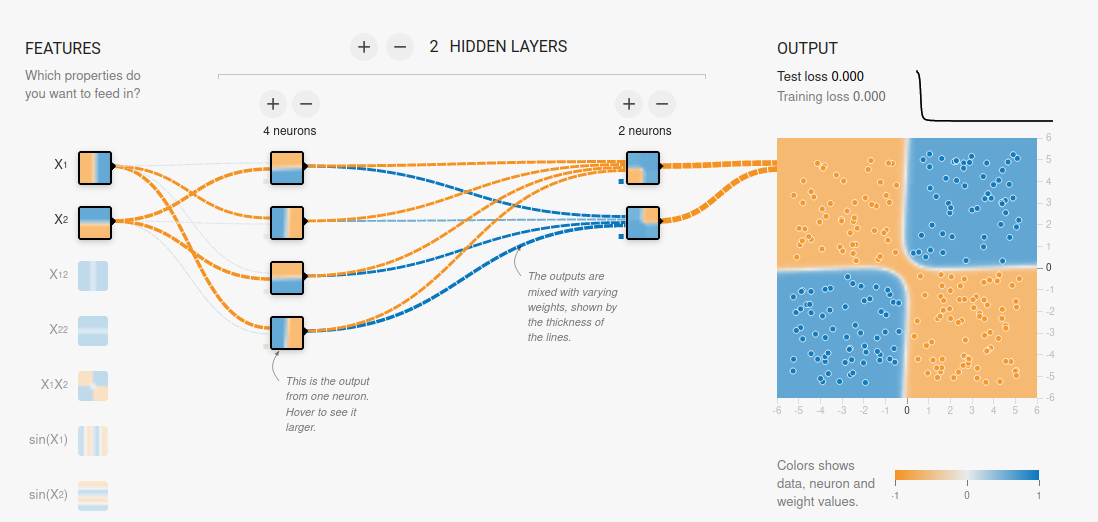
\includegraphics[width=0.9\textwidth]{figs/playground.png}
\end{frame}

\section{Deep Learning}

\begin{frame}{Deep Learning (I)}
    Deep Learning is not just a network with many layers
	\begin{itemize}
        \item High number of parameters to optimize
		\item More layers $\Rightarrow$ more local optima $\Rightarrow$ more difficult training
	\item Large datasets
	\item Gradient vanishing / exploding

	\medskip
	\centering
	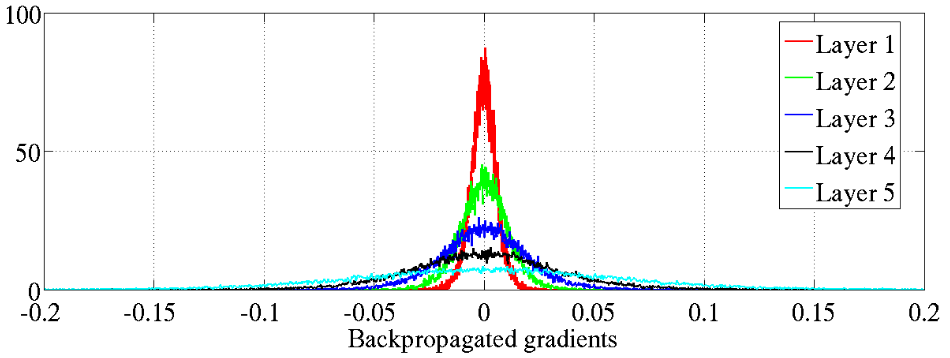
\includegraphics[width=0.7\textwidth]{figs/gradients.png}\\
	%\scriptsize\href{http://proceedings.mlr.press/v9/glorot10a/glorot10a.pdf?source=post\_page---------------------------}{(Source)}\\
	\end{itemize}
\end{frame}

\begin{frame}{Deep Learning (II)}
	Need of tricks to train deep networks
	\begin{itemize}
		\item Careful weights initialization
			\begin{itemize}
			\item Glorot and He initialization, LeCun initialization
			\end{itemize}
		\item Non-saturating activation functions
			\begin{itemize}
			\item Sigmoid activation is problematic
			\item ReLU and Leaky ReLU activation functions
			\end{itemize}
		\item Batch normalization
		\item Transfer learning/ pretained models
	\end{itemize}
		\centering 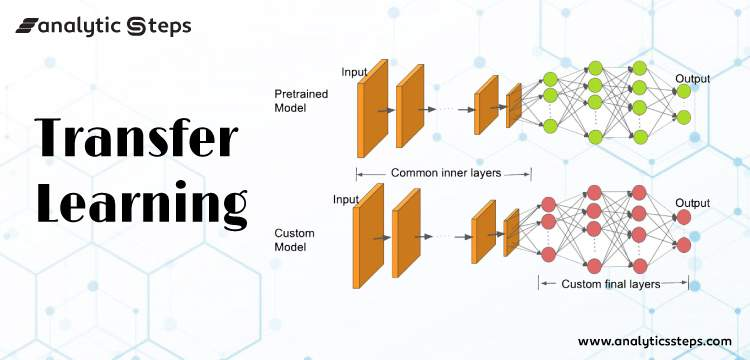
\includegraphics[width=0.7\textwidth]{figs/transfer.jpg}\\
	\scriptsize\href{https://www.analyticssteps.com/blogs/how-transfer-learning-done-neural-networks-and-convolutional-neural-networks}{(Source)}\\
\end{frame}

\begin{frame}{Deep Learning (III)}
    \begin{columns}
 	   \column{.50\textwidth}
		\begin{itemize}
		\item Unsupervised pretraining
		\item Regularization
			\begin{itemize}
				\item L1, L2 and \alert{dropout}
			\end{itemize}
		\item Faster optimizers
			\begin{itemize}
				\item AdaGrad, Adam, RMSProp
			\end{itemize}
		\item \alert{Data augmentation} 
			\begin{itemize}
				\item Creates modified copies of the dataset
				\item It increases the number of samples
			\end{itemize}
        	\item Clever design of the network to minimize parameters
	\end{itemize}

 	   \column{.50\textwidth}
	    	\centering 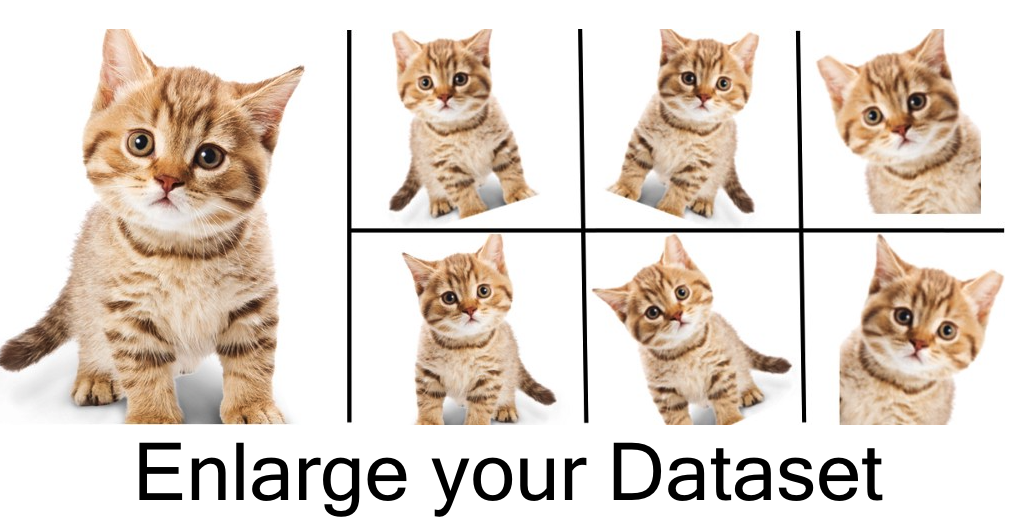
\includegraphics[width=\linewidth]{figs/augmentation.png}\\
	    \scriptsize\href{https://medium.com/nanonets/how-to-use-deep-learning-when-you-have-limited-data-part-2-data-augmentation-c26971dc8ced}{(Source)}\\
    \end{columns}
\end{frame}

\begin{frame}{Deep Learning (IV)}
	In Deep Learning, we use to think in layers
	\begin{itemize}
		\item Data input layers
		\item Output layers
        	\item Fully connected (classic)
        	\item Convolutional layers
        	\item Max-pooling
        	\item Recurrent layers
        	\item Dropout layers
        	\item More ...
	\end{itemize}

    \vspace{-3.5cm}
	\hfill 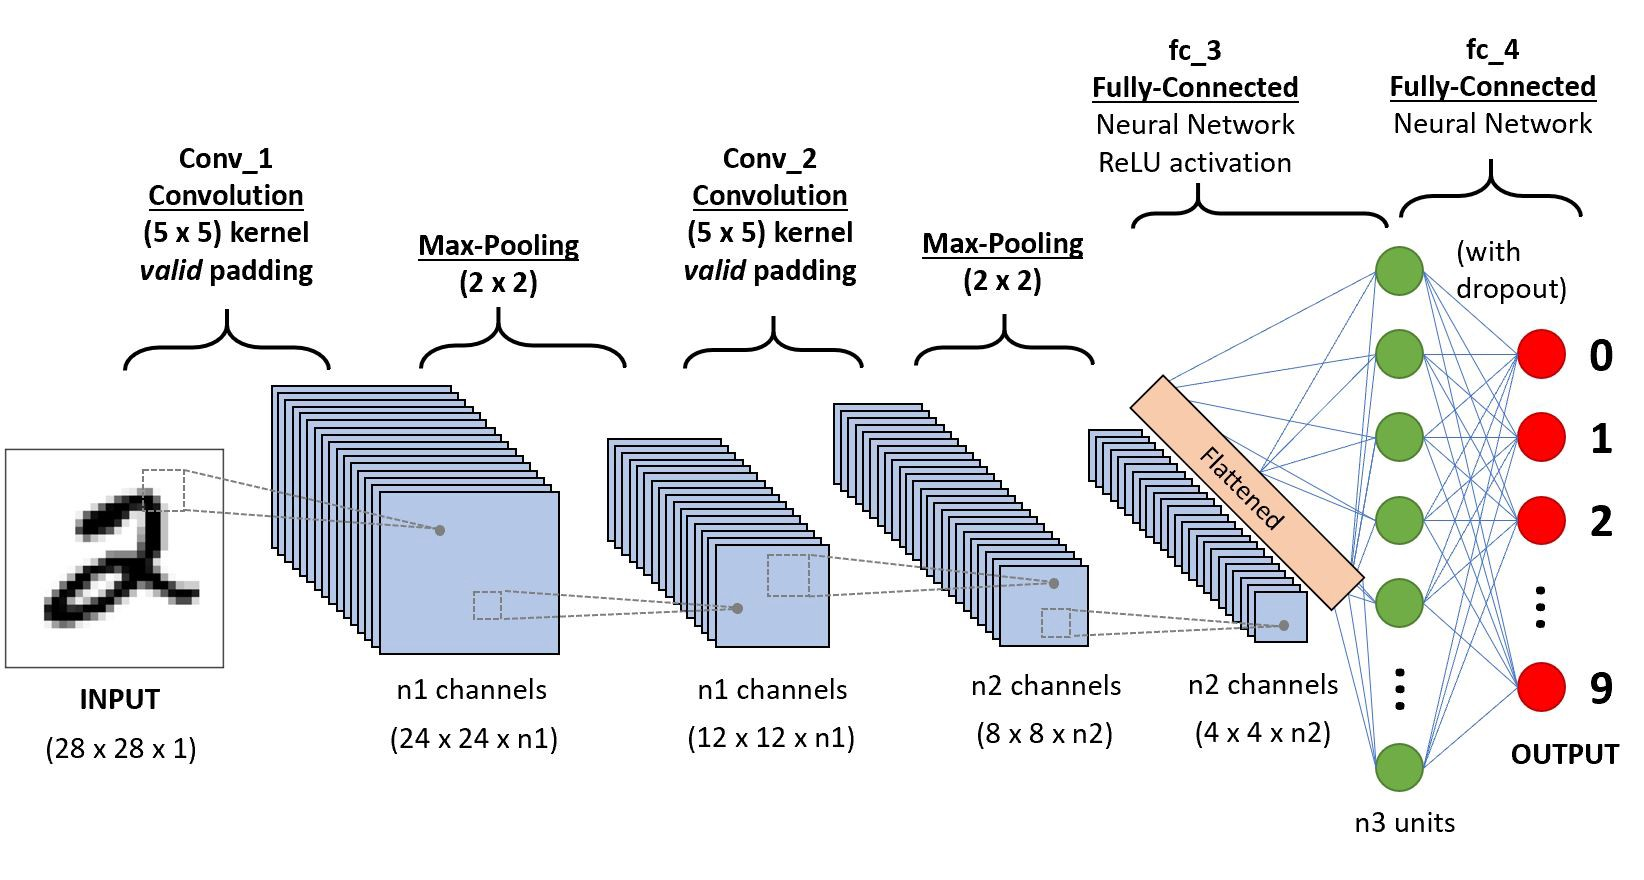
\includegraphics[width=0.6\textwidth]{figs/layers.png}\\
	%\scriptsize\href{https://towardsdatascience.com/a-comprehensive-guide-to-convolutional-neural-networks-the-eli5-way-3bd2b1164a53}{(Source)}\\

	Two popular types of deep architectures
	\begin{itemize}
		\item Convolutional Neural Networks (CNNs) - Image processing
		\item Long Short-Term Memory (LSTM) - Time-series and NLP 
	\end{itemize}
\end{frame}

\section{Convolutional Neural Networks}
\subsection{Biological motivation}
\begin{frame}{Convolutional Neural Networks}{Biological motivation}
	\centering
	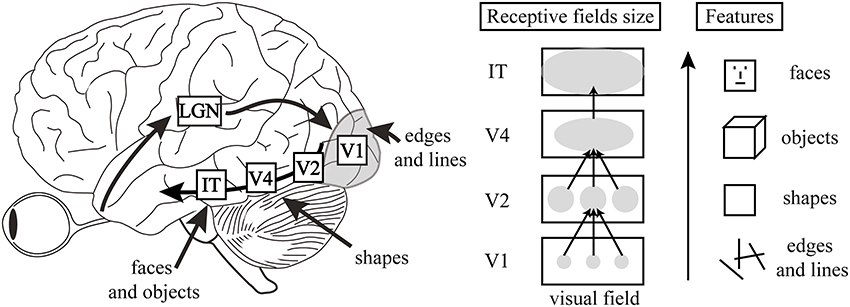
\includegraphics[width=0.9\textwidth]{figs/cortex.png}\\
	\scriptsize\href{https://www.researchgate.net/publication/267872860_Why_vision_is_not_both_hierarchical_and_feedforward/figures?lo=1}{(Source)}\\
\end{frame}

\subsection{Convolutional layer}
\begin{frame}{Convolutional Neural Networks}{Convolutional layers (I)}
    CNNs are popular for Computer Vision applications
	\begin{itemize}
		\item Networks with convolutional layers
        \item Convolutions are features extrators
        \item Its behaviour can be learnt
	\end{itemize}

    %\bigskip 
%	\centering 1D convolution \\
%    \bigskip 

%	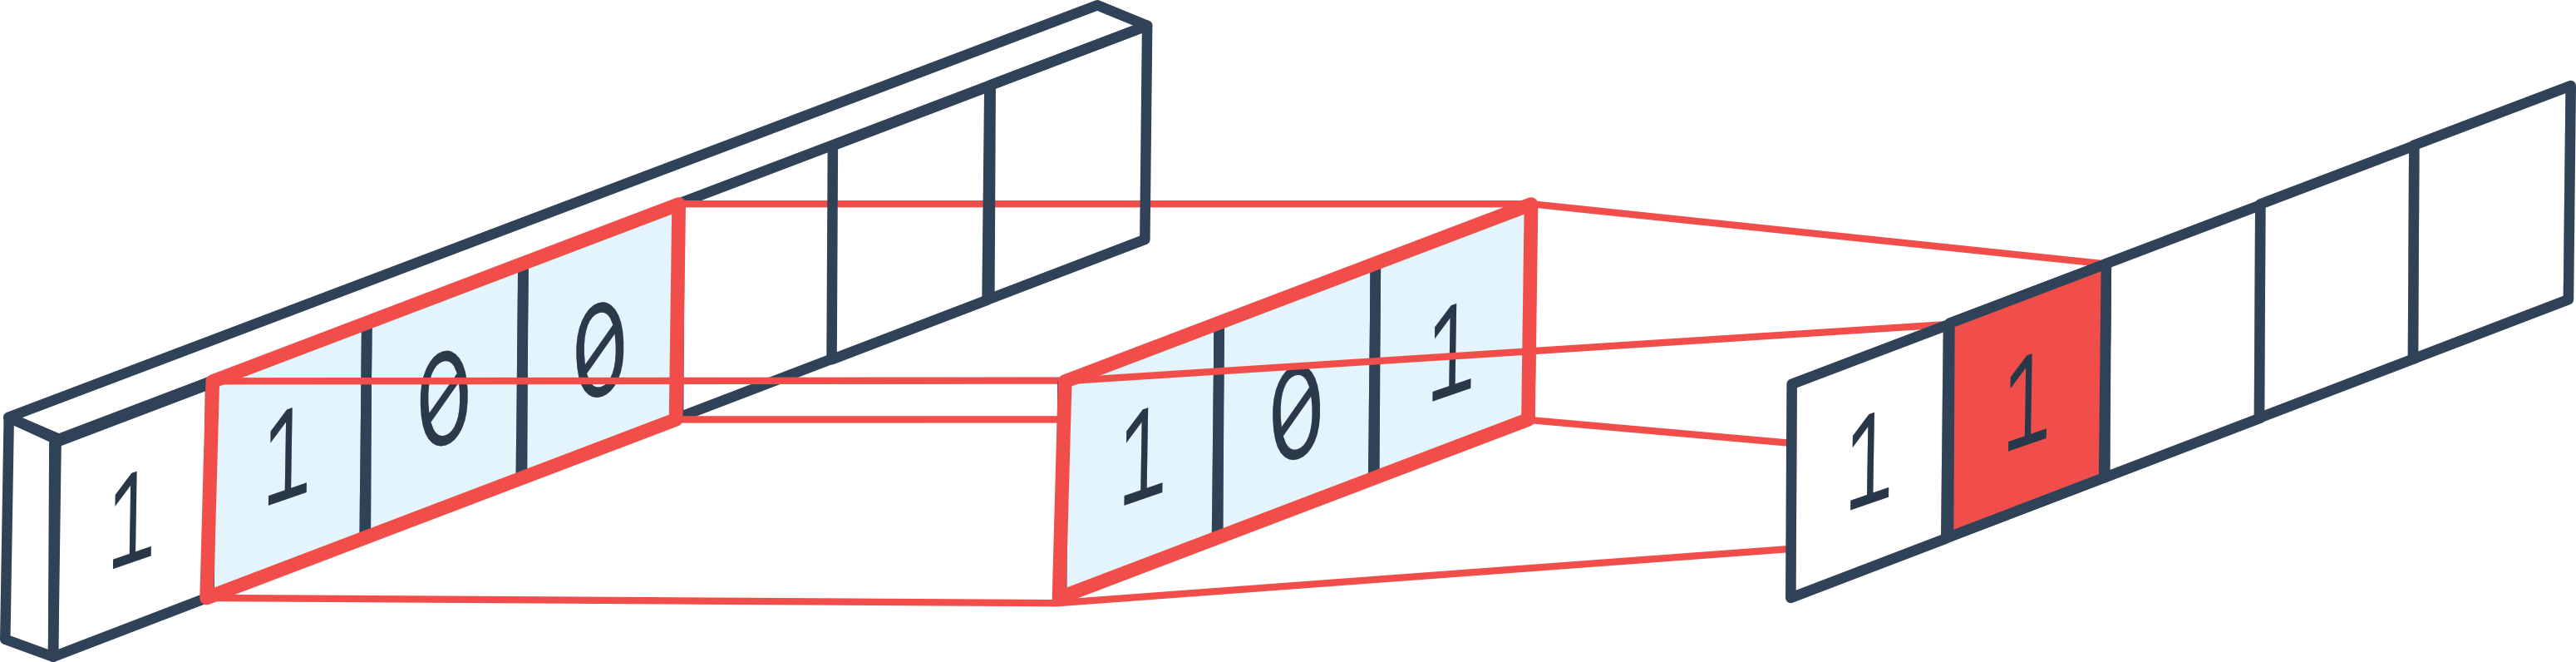
\includegraphics[width=0.5\textwidth]{figs/1dconv.png}
\end{frame}

\begin{frame}{Convolutional Neural Networks}{Convolutional layers (II)}
    \centering

	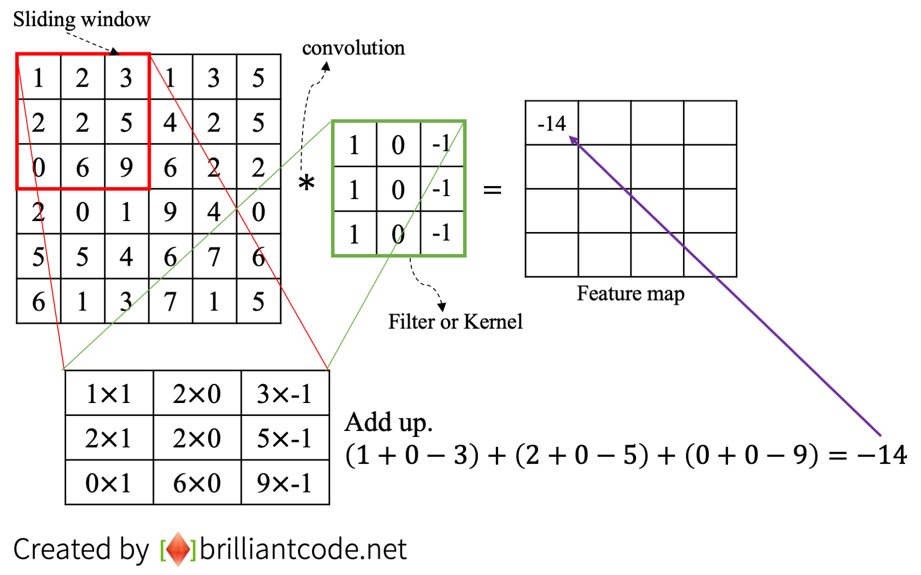
\includegraphics[width=0.8\textwidth]{figs/2dconvolution.png}\\
	\scriptsize\href{https://www.brilliantcode.net/1584/convolutional-neural-networks-1-convolution-layer-stride-padding-kernel/}{(Source)}\\
    \bigskip
	\normalsize \href{https://miro.medium.com/max/500/1*GcI7G-JLAQiEoCON7xFbhg.gif}{(Conv 2D example)}
\end{frame}

\begin{frame}{Convolutional Neural Networks}{Convolutional layers (III)}

    \begin{columns}
 	\column{.50\textwidth}
	    \centering Padding\\
        \bigskip
	    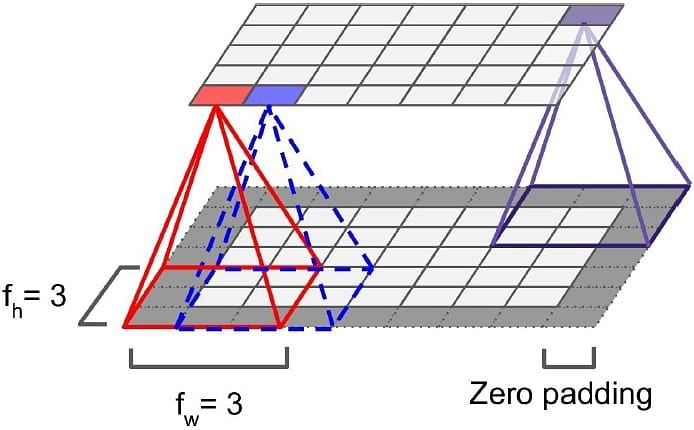
\includegraphics[width=\textwidth]{figs/padding.png}\\
    	\scriptsize\href{https://www.oreilly.com/library/view/hands-on-machine-learning/9781492032632/}{(Source)}

 	\column{.50\textwidth}
        \centering Stride\\
        \bigskip
	    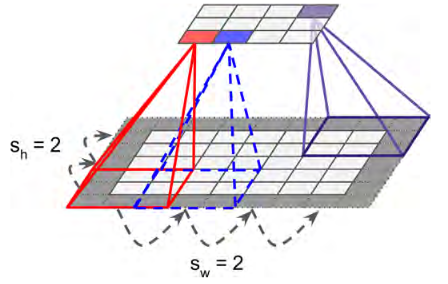
\includegraphics[width=\textwidth]{figs/stride.png}\\
	    \scriptsize\href{https://www.oreilly.com/library/view/hands-on-machine-learning/9781492032632/}{(Source)}
    \end{columns}
\end{frame}

\begin{frame}{Convolutional Neural Networks}{Convolutional layers (IV)}
	\centering
	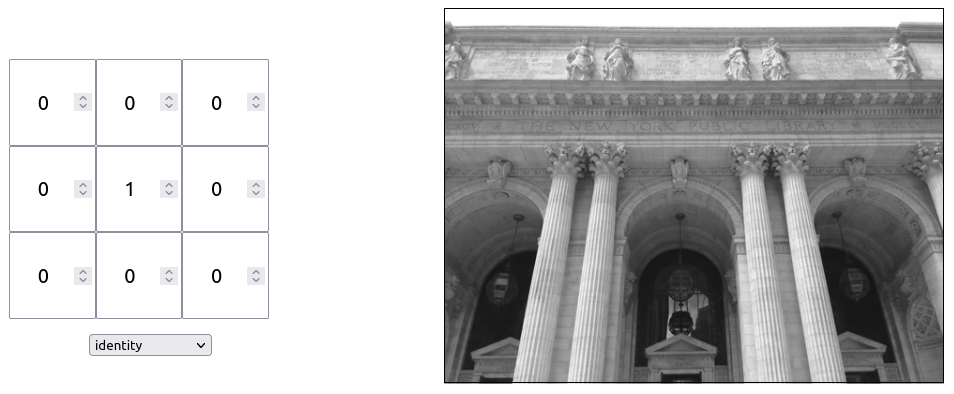
\includegraphics[width=0.5\textwidth]{figs/convolution1.png}\\\bigskip
	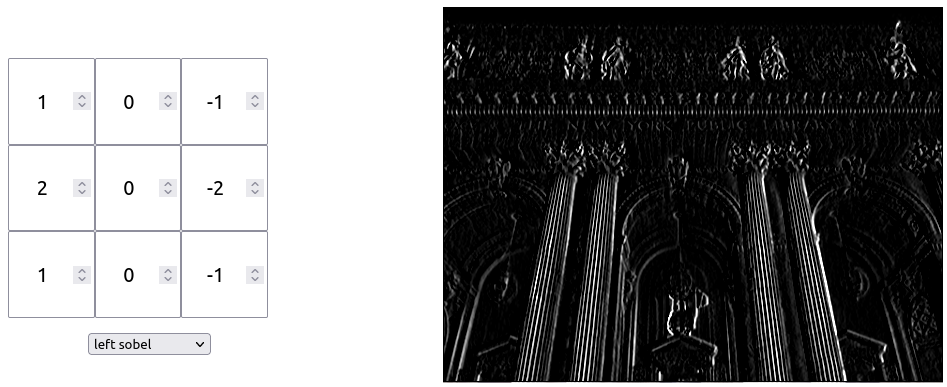
\includegraphics[width=0.45\textwidth]{figs/convolution2.png}
	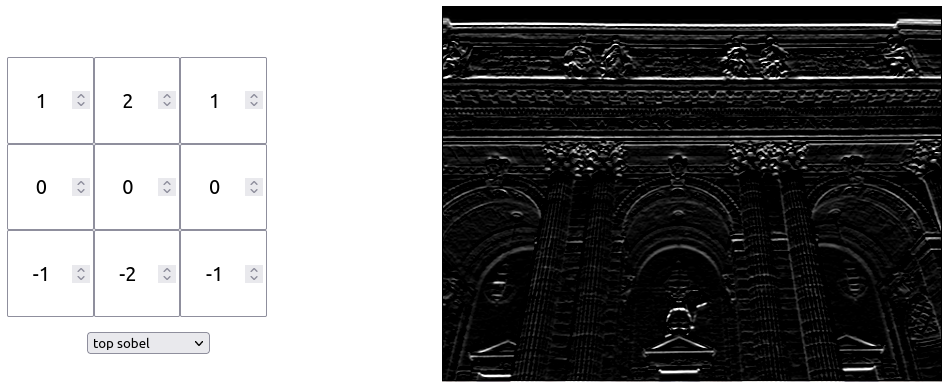
\includegraphics[width=0.45\textwidth]{figs/convolution3.png}\\
    \bigskip
    \href{https://setosa.io/ev/image-kernels/}{(Image kernels)}
\end{frame}

\subsection{Max-pooling layer}
\begin{frame}{Convolutional Neural Networks}{Max-pooling layer}
	\centering{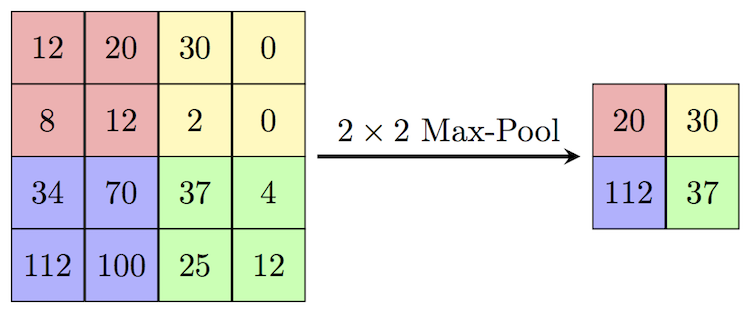
\includegraphics[width=0.5\textwidth]{figs/maxpool.png}}

    \bigskip

    \begin{flushleft}
    Max-pooling down-samples data instances
	\begin{itemize}
		\item Given a matrix, it takes its maximum value
		\item Usually the matrix is $n x n$ (2D)
	\end{itemize}
	Benefits
	\begin{itemize}
		\item Dimensionality reduction
		\item Filters irrelevant information
        \item Invariant to scale
	\end{itemize}
    \end{flushleft}
\end{frame}

\subsection{Dropout layer}
\begin{frame}{Convolutional Neural Networks}{Dropout layer}
	\alert{Dropout} is a regularization technique for neural networks
	\begin{itemize}
		\item Dropout deactivates a neuron with probability $p$ for each iteration
	\end{itemize}

	Related concept: \alert{dense layers}
	\begin{itemize}
		\item In Keras, it is just a fully connected layer with regular neurons
	\end{itemize}
	\centering
        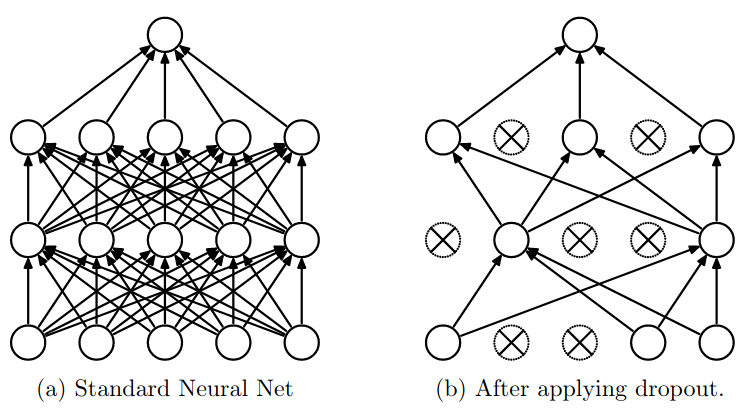
\includegraphics[width=0.6\textwidth]{figs/dropout.png}\\
	\scriptsize\href{https://jmlr.org/papers/volume15/srivastava14a.old/srivastava14a.pdf}{(Srivastava et al. (2010))}
\end{frame}

\subsection{CNN architectures}
\begin{frame}{Convolutional Neural Networks}{CNN architectures: standard (I)}
	\centering
        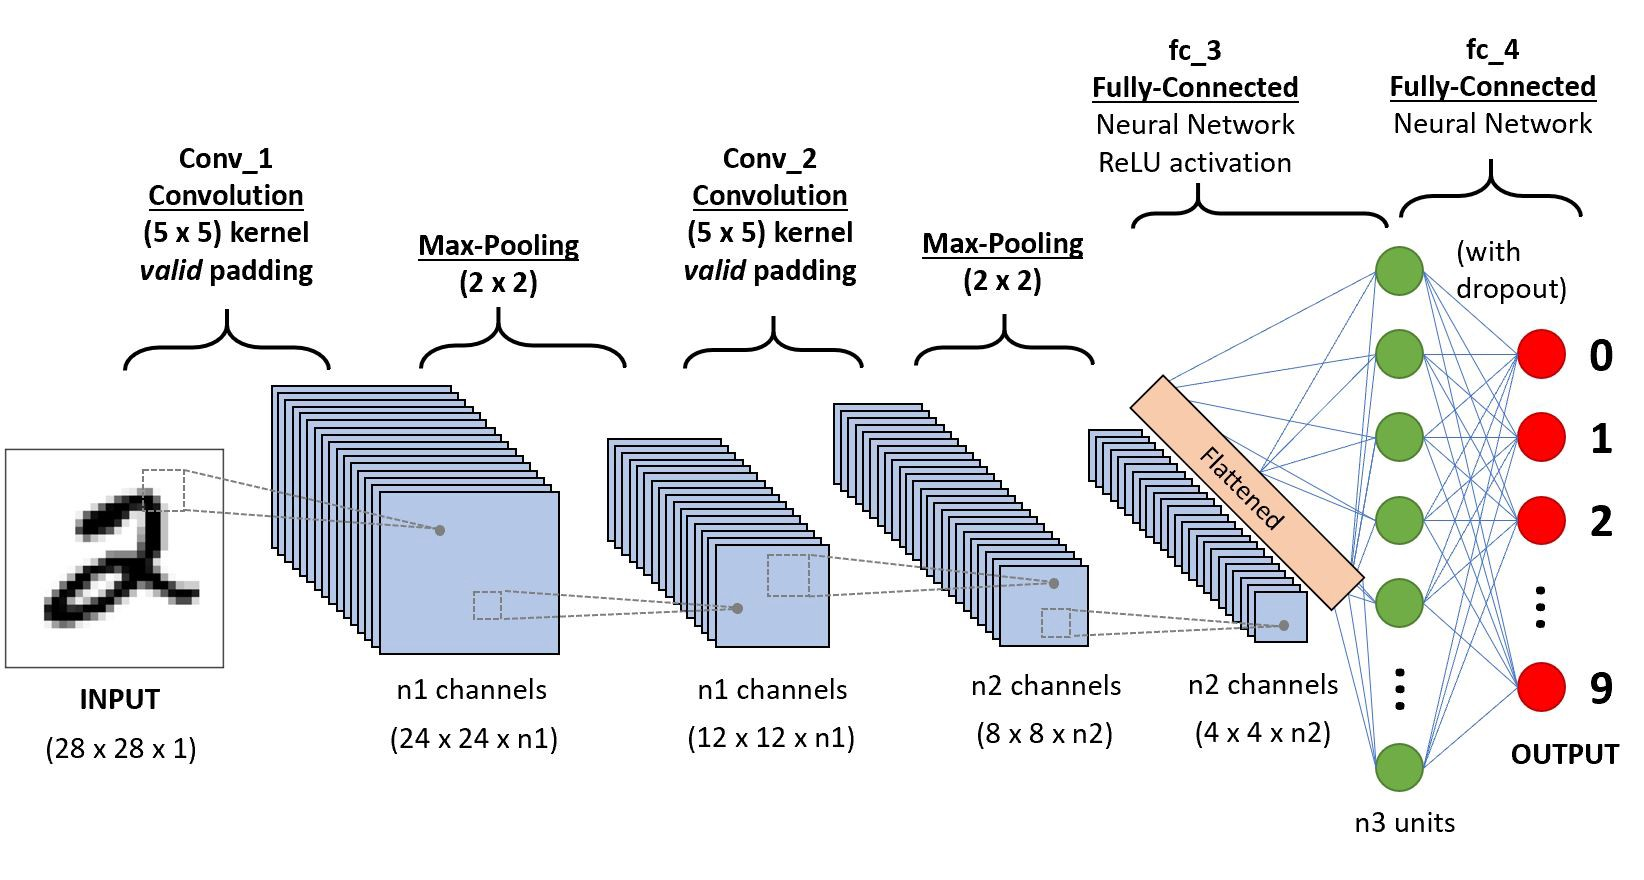
\includegraphics[width=\textwidth]{figs/layers.png}\\
	    \scriptsize\href{https://towardsdatascience.com/a-comprehensive-guide-to-convolutional-neural-networks-the-eli5-way-3bd2b1164a53}{(Source)}\\

	\normalsize \href{https://poloclub.github.io/cnn-explainer/}{(Demo)}
\end{frame}

{\blackSlide
\begin{frame}{Convolutional Neural Networks}{CNN architectures: standard (II)}
	\centering
        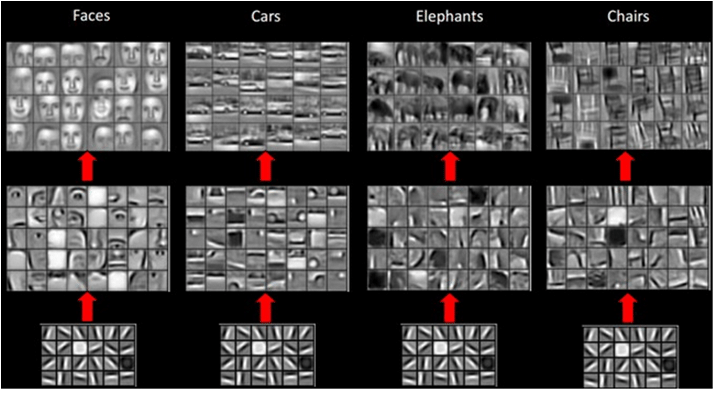
\includegraphics[width=0.9\textwidth]{figs/features.png}
\end{frame}
}

\subsubsection{Other CNN architectures}
\begin{frame}{Convolutional Neural Networks}{Other CNN architectures}
    \begin{columns}
 	   \column{.30\textwidth}
    Other CNN architectures
    \begin{itemize}
        \item LeNet-5
        \item AlexNet
        \item GoogLeNet
        \item VGGNet
        \item ResNet
        \item Xception
        \item SENet
    \end{itemize}

 	   \column{.70\textwidth}
	Performance on Imagenet
	    \smallskip
    \begin{tabular}{l|l|l|l}
    Model & Acc. & Parameters & Depth\\\hline
    VGG16       & $0.901$ & $138.357.544$ & 23 \\
    InceptionV3 & $0.937$ & $23.851.784$ & 159 \\
    ResNet50    & $0.921$ & $25.636.712$ & -   \\
    Xception    & $0.945$ & $22.910.480$ & 126 \\
    \end{tabular}

    \bigskip

    Famous generative deep networks
    \smallskip
    \begin{tabular}{l|l}
    Model & Parameters  \\\hline
    GTP-2 & 1.5 billion (1,500,000,000) \\
    GTP-3 & 175 billion (175,000,000,000) \\
    Dall-E 2& 12 billion (12.000.000.000) \\
    ChatGPT& Unknown\\
    \end{tabular}

    \end{columns}
\end{frame}

\subsection{Classification and localization}
\begin{frame}{Convolutional Neural Networks}{Classification and localization}
	Localization: Predict a bounding box around the object
    	\begin{itemize}
    		\item Classification as a regression problem: X, Y, width and height
        	\item Four output units per class
    	\end{itemize}

    We need annotation tools
    \begin{itemize}
	    \item \href{https://www.robots.ox.ac.uk/~vgg/software/via/}{(VGG Image annotator)}, \href{https://github.com/heartexlabs/labelImg}{(LabelImg)}, \href{(https://imglab.in/)}{(ImgLab)}	
    \end{itemize}

    \begin{columns}
 	   \column{.10\textwidth}
 	   \column{.4\textwidth}
        	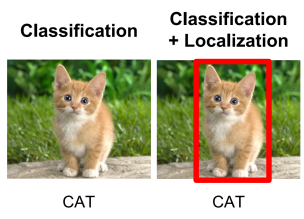
\includegraphics[width=\textwidth]{figs/localization-2.png}
 	   \column{.05\textwidth}
 	   \column{.35\textwidth}
        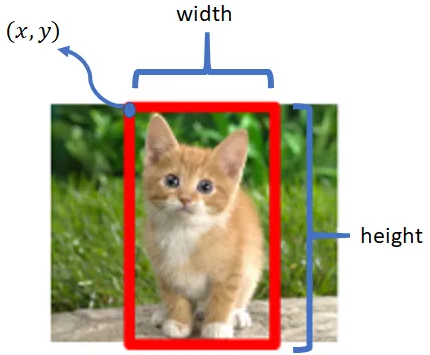
\includegraphics[width=\textwidth]{figs/localization.png}
 	   \column{.10\textwidth}
    \end{columns}
	    \centering
	\scriptsize\href{https://medium.com/@rajshekhar_k/object-localization-series-2-1-basic-object-classification-with-localization-3c8e35fbd0f1}{(Source)}
\end{frame}

\subsection{Object detection}
\begin{frame}{Convolutional Neural Networks}{Object detection}
	\flushleft Object detection: Classify and localize multiple objects in an image \\ 
        \centering 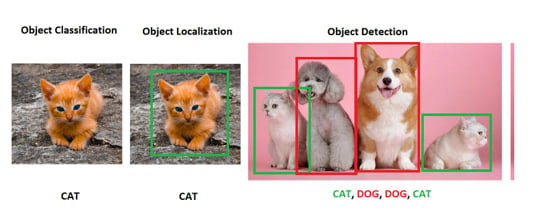
\includegraphics[width=0.6\textwidth]{figs/detection.jpg}\\
	\scriptsize\href{https://dev.to/sally20921/basics-of-object-detection-part-1-1i52}{(Source)}

	\normalsize

    \begin{columns}
 	   \column{.60\textwidth}
	\flushleft Old approach: Slide across a single object CNN\\
	\begin{itemize}
		\item The image must pass through the CNN several times
		\item Bad for real-time applications
	\end{itemize}
        
 	   \column{.40\textwidth}
        \centering 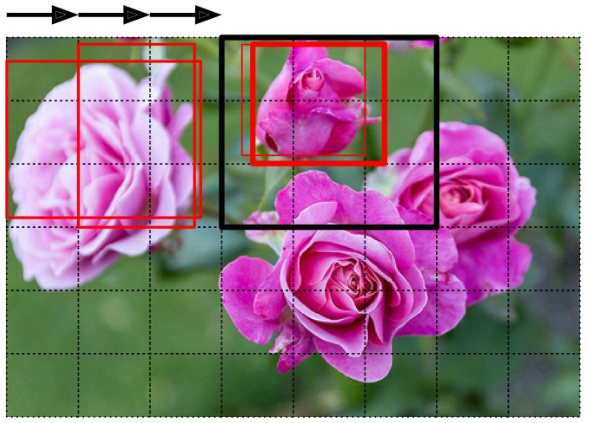
\includegraphics[width=\textwidth]{figs/object}\\
	\scriptsize\href{http://powerunit-ju.com/wp-content/uploads/2021/04/Aurelien-Geron-Hands-On-Machine-Learning-with-Scikit-Learn-Keras-and-Tensorflow_-Concepts-Tools-and-Techniques-to-Build-Intelligent-Systems-OReilly-Media-2019.pdf}{(Source)}
    \end{columns}
\end{frame}

\subsubsection{Object detection: You Only Look Once (YOLO)}
\begin{frame}{Convolutional Neural Networks}{Object detection: You Only Look Once (YOLO)}
    \begin{columns}
 	   \column{.60\textwidth}
	YOLO is a fast architecture for real-time object detection
	\begin{itemize}
		\item Several versions proposed by different teams
		\item Valid for video object detection
		\item Several implementations
		\item \href{https://github.com/ultralytics/ultralytics}{(Yolo v8)}
		\item YOLO supports image segmentation
	\end{itemize}

 	   \column{.40\textwidth}
        \centering 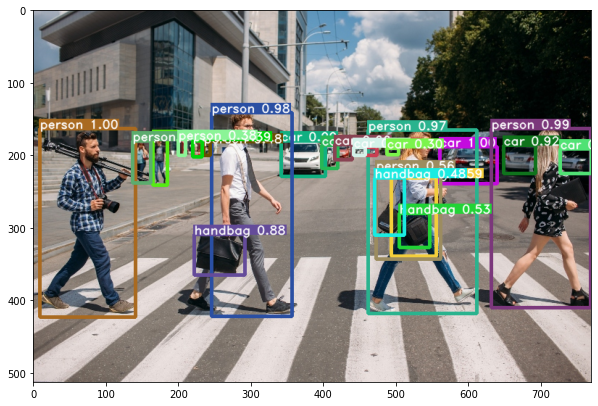
\includegraphics[width=\textwidth]{figs/yolo-pedestrians.png}\\
	\scriptsize\href{https://neptune.ai/blog/object-detection-with-yolo-hands-on-tutorial}{(Source)}\\

        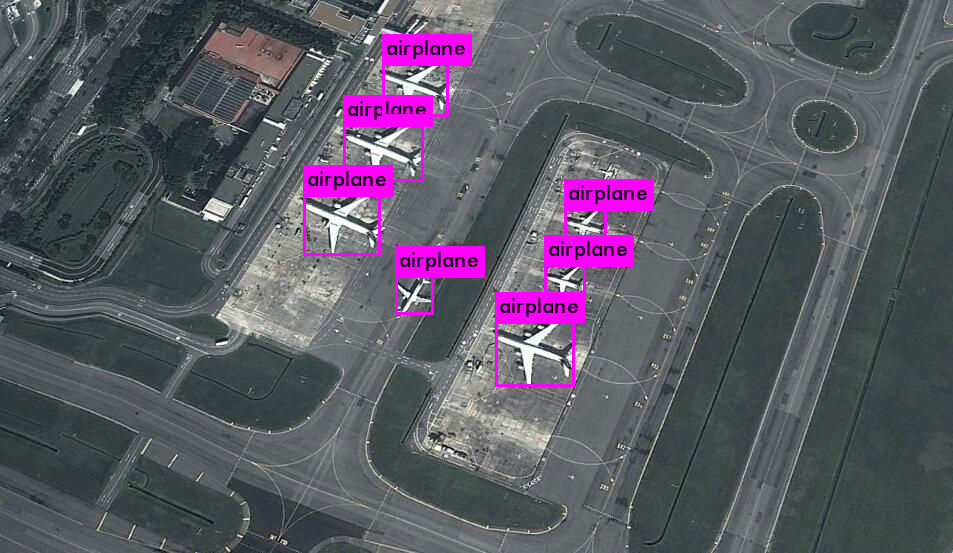
\includegraphics[width=\textwidth]{figs/yolov3.jpg}\\
	\scriptsize\href{https://github.com/yoyotv/YOLO-project}{(Source)}\\
    \end{columns}
\end{frame}

\subsection{Semantic segmentation}
\begin{frame}{Convolutional Neural Networks}{Semantic segmentation}
    \begin{columns}
 	   \column{.60\textwidth}
	\flushleft
	Semantic segmentation: Pixel-level classification
	\medskip
	\centering
        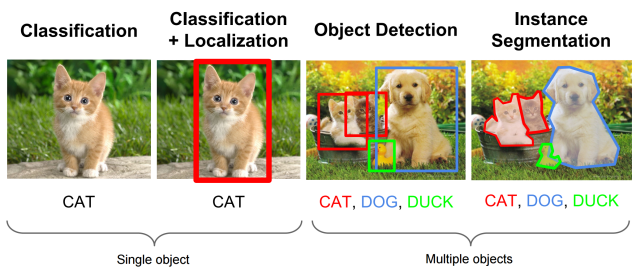
\includegraphics[width=\textwidth]{figs/segmentation.png}\\
	\scriptsize\href{https://towardsdatascience.com/object-localization-in-overfeat-5bb2f7328b62}{(Source)}\\

 	   \column{.40\textwidth}
    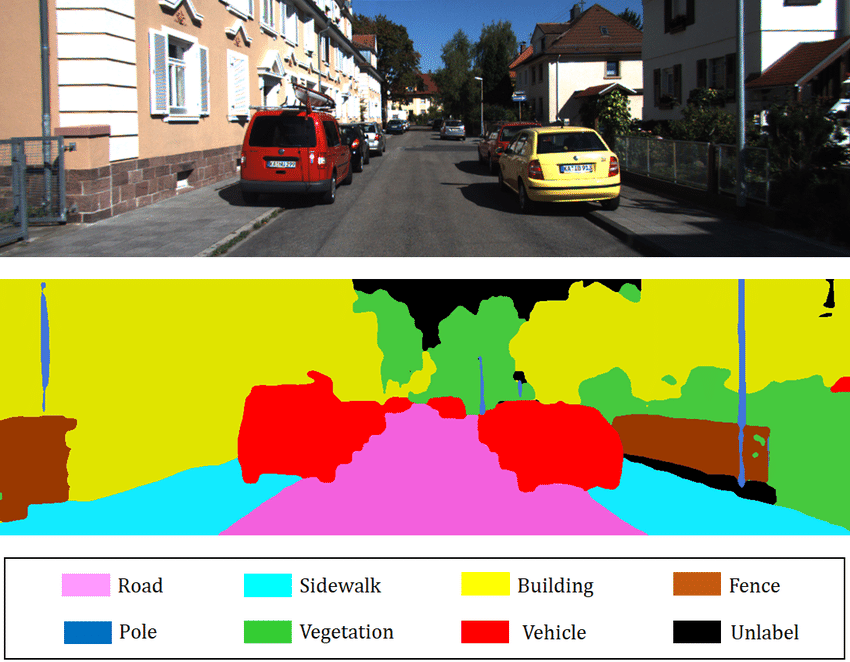
\includegraphics[width=\linewidth]{figs/semantic.png}\\
	    \centering
    \scriptsize\href{https://www.researchgate.net/figure/Example-of-2D-semantic-segmentation-Top-input-image-Bottom-prediction_fig3_326875064}{(Source)}\\
	\end{columns}
\end{frame}



\section{Recurrent networks}
\subsection{RNNs}
\begin{frame}{Recurrent networks}{Recurrent neural networks (I)}
    %\begin{columns}
 	%   \column{.50\textwidth}
	Recurrent networks have connections pointing backward
    \begin{itemize}
        \item Time-series, NLP, audio, video, ...
    \end{itemize}
    Neurons have memory, or \textbf{state}
    \begin{itemize}
        \item Named \alert{cells}
        \item In basic neurons, state and output are the same
    \end{itemize}

	\begin{figure}
        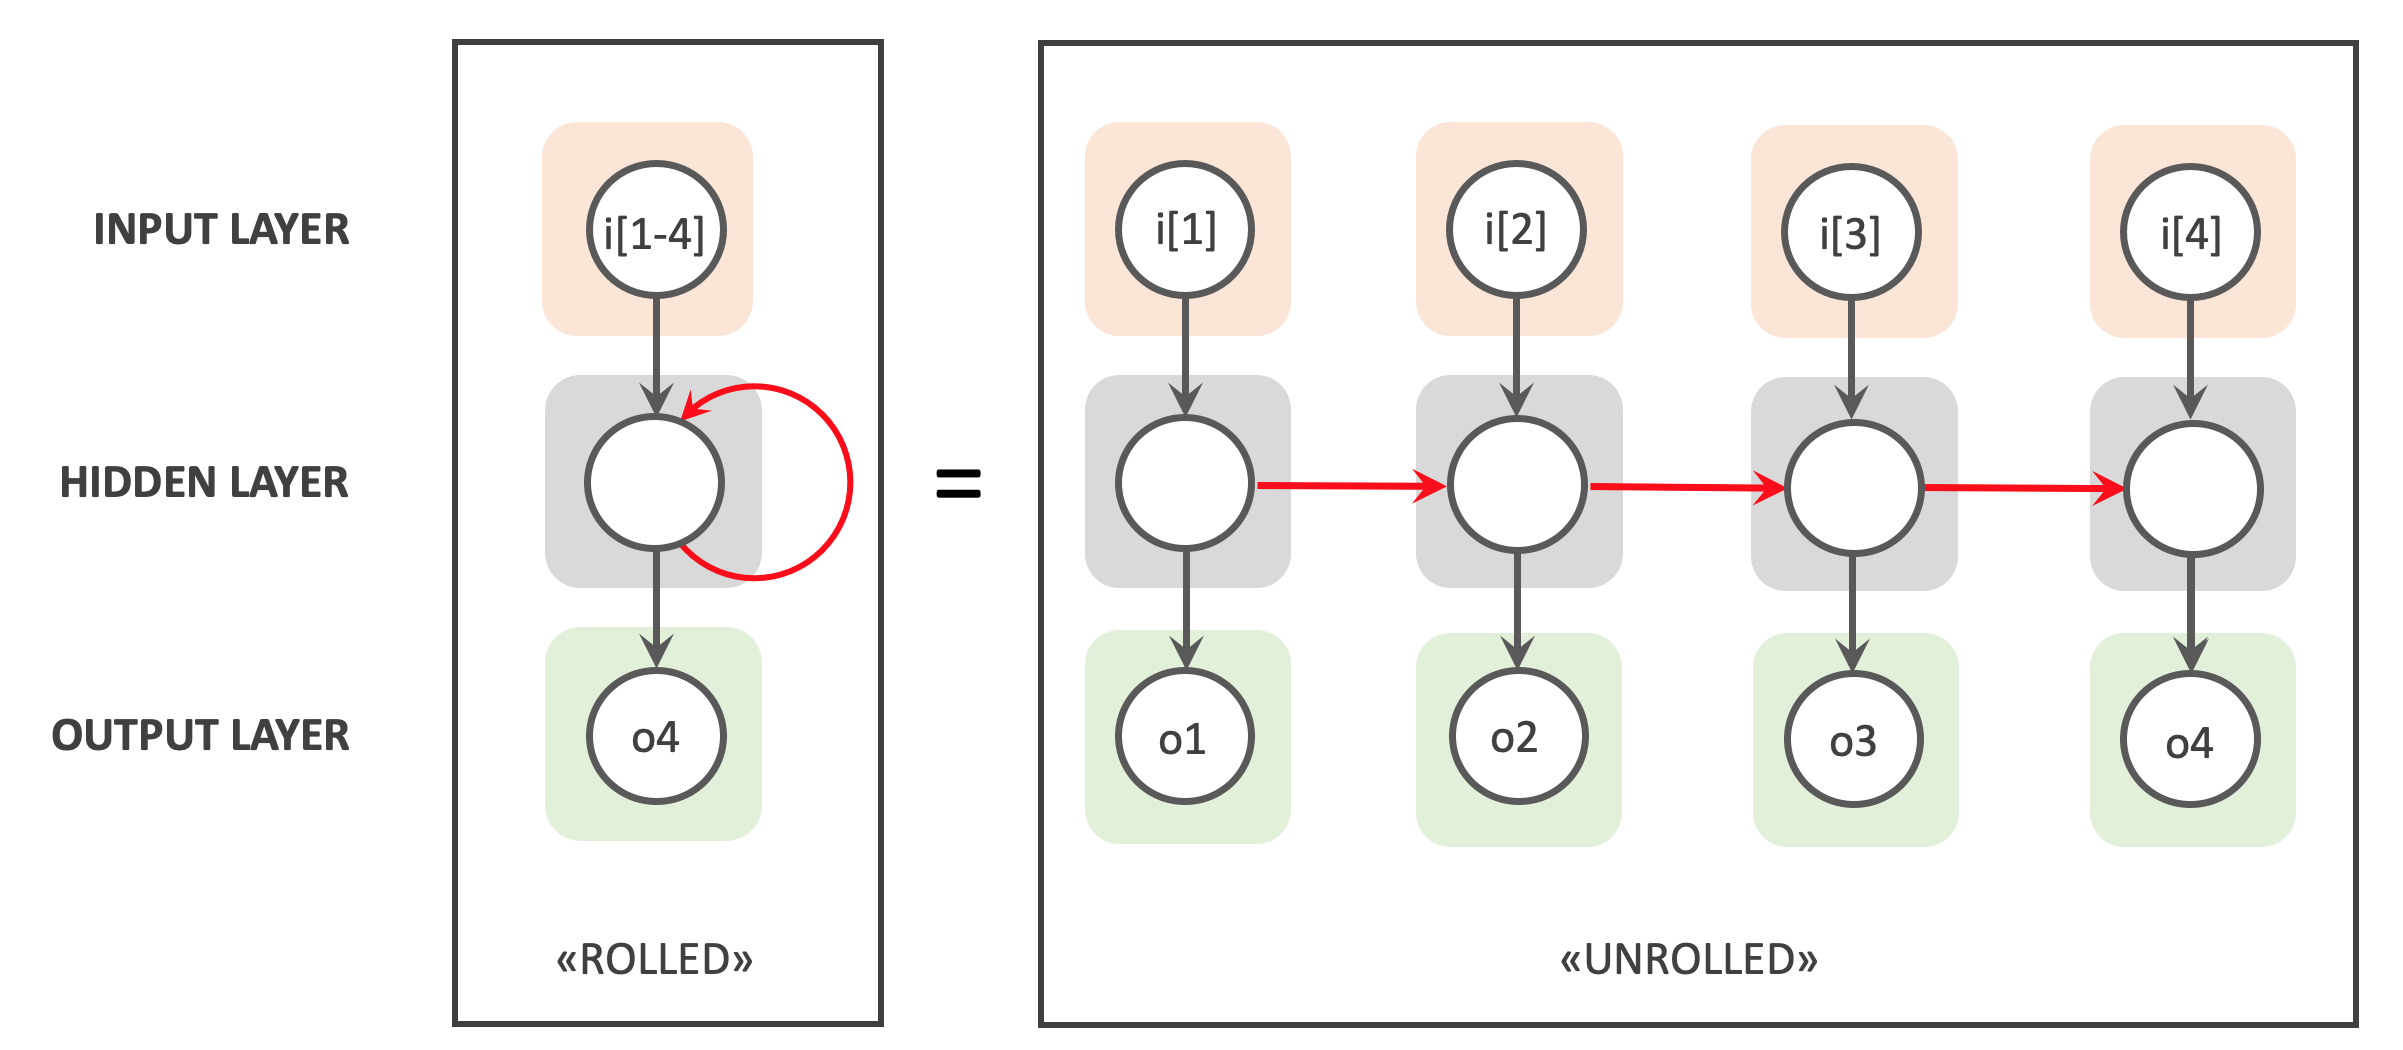
\includegraphics[width=0.6\textwidth]{figs/recurrent.png}\\
	    \scriptsize\href{https://www.bouvet.no/bouvet-deler/explaining-recurrent-neural-networks}{(Source)}
	\end{figure}
\end{frame}

\begin{frame}{Recurrent networks}{Recurrent neural networks (II)}
	\centering
    Sequence learning
    \bigskip
        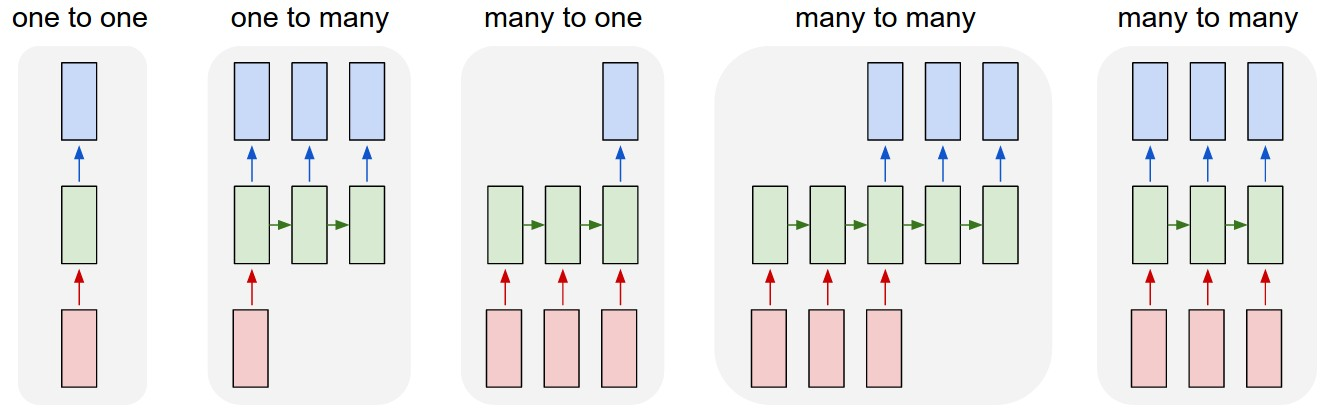
\includegraphics[width=0.8\textwidth]{figs/seq2seq.jpg}

    \begin{table}
    \centering
    \begin{tabular}{l|l|l}
    One to many & Many to one & Many to many\\
    vec2seq     & seq2vec     & seq2seq\\\hline
    Image description & Spam classification & Machine translation \\
                & Time series forecasting & \\
                & Sentiment score         & \\
    \end{tabular}
    \end{table}
\end{frame}



\begin{frame}{Recurrent networks}{Recurrent neural networks (III)}
    RNNs problems
    \begin{itemize}
        \item Gradient unstability
            \begin{itemize}
            \item Smaller learning rate
            \item tanh as activation function
            \item Usual DL tricks
            \end{itemize}
        \item Short memory
            \begin{itemize}
            \item Information vanishes fast
            \item Much more difficult solution
            \end{itemize}
    \end{itemize}
\end{frame}

\subsection{LTSM networks}
\begin{frame}{Recurrent networks}{LSTM networks}
    \begin{columns}
 	   \column{.50\textwidth}
            LSTM: Long-Short Term Memory
            \begin{itemize}
                \item Complex cell that improves long-term memory
                \item Two states: short and long terms
                \item Very much used as a basic cell
                \item Much better performance
                \item Lower training time
            \end{itemize}
 	   \column{.50\textwidth}
            \centering 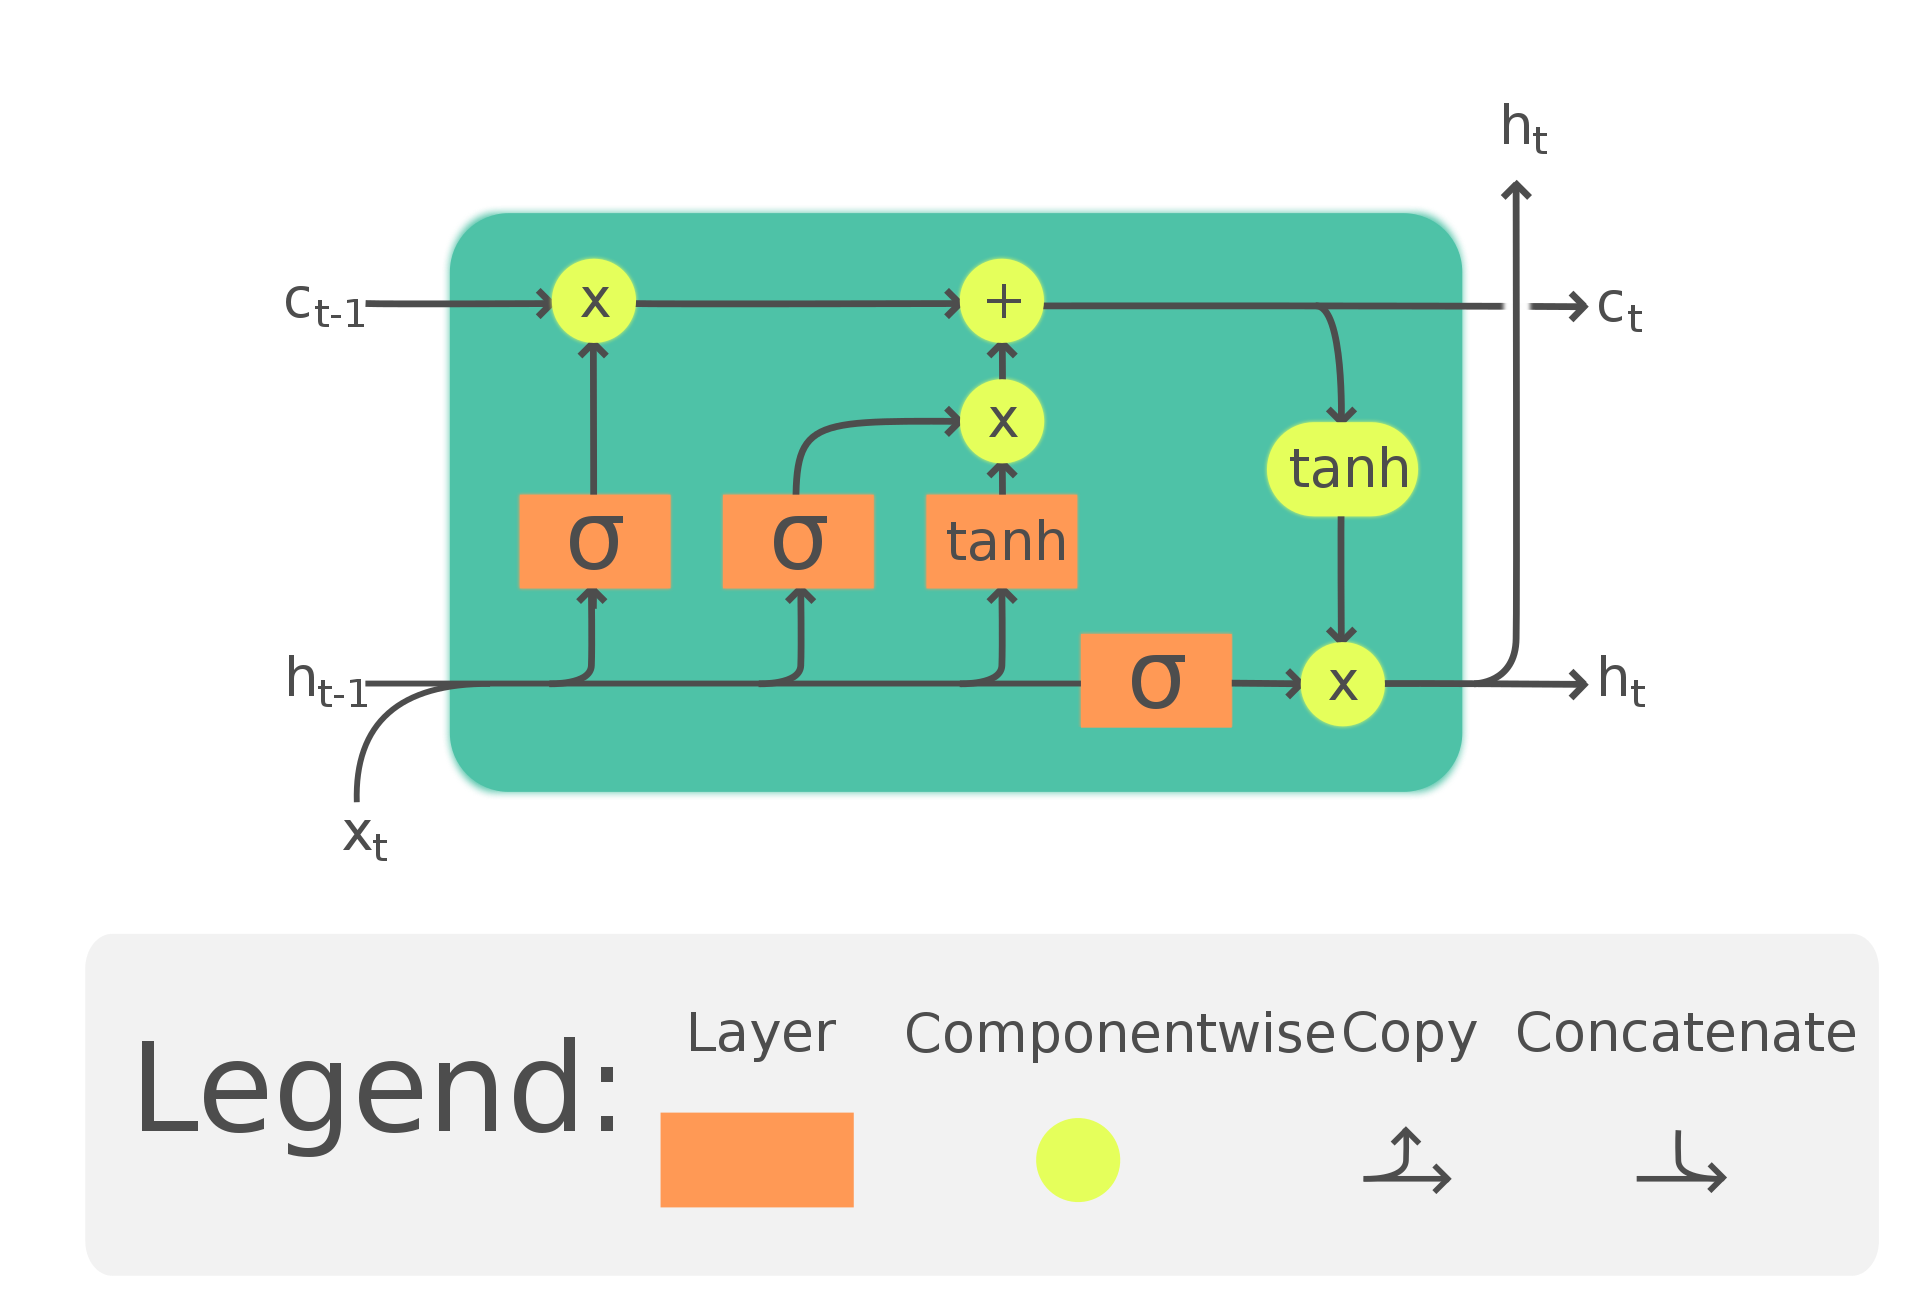
\includegraphics[width=\textwidth]{figs/LTSM.png}\\
	        \scriptsize\href{https://en.wikipedia.org/wiki/Long_short-term_memory}{(Source)}
    \end{columns}
\end{frame}

\subsection{GRU networks}
\begin{frame}{Recurrent networks}{GRU}
    \begin{columns}
 	   \column{.50\textwidth}
            GRU: Gated Recurrent Unit
            \begin{itemize}
                \item Simplification of LSTM
                \item Seems to perform as well as LSTM
            \end{itemize}
 	   \column{.50\textwidth}
            \centering 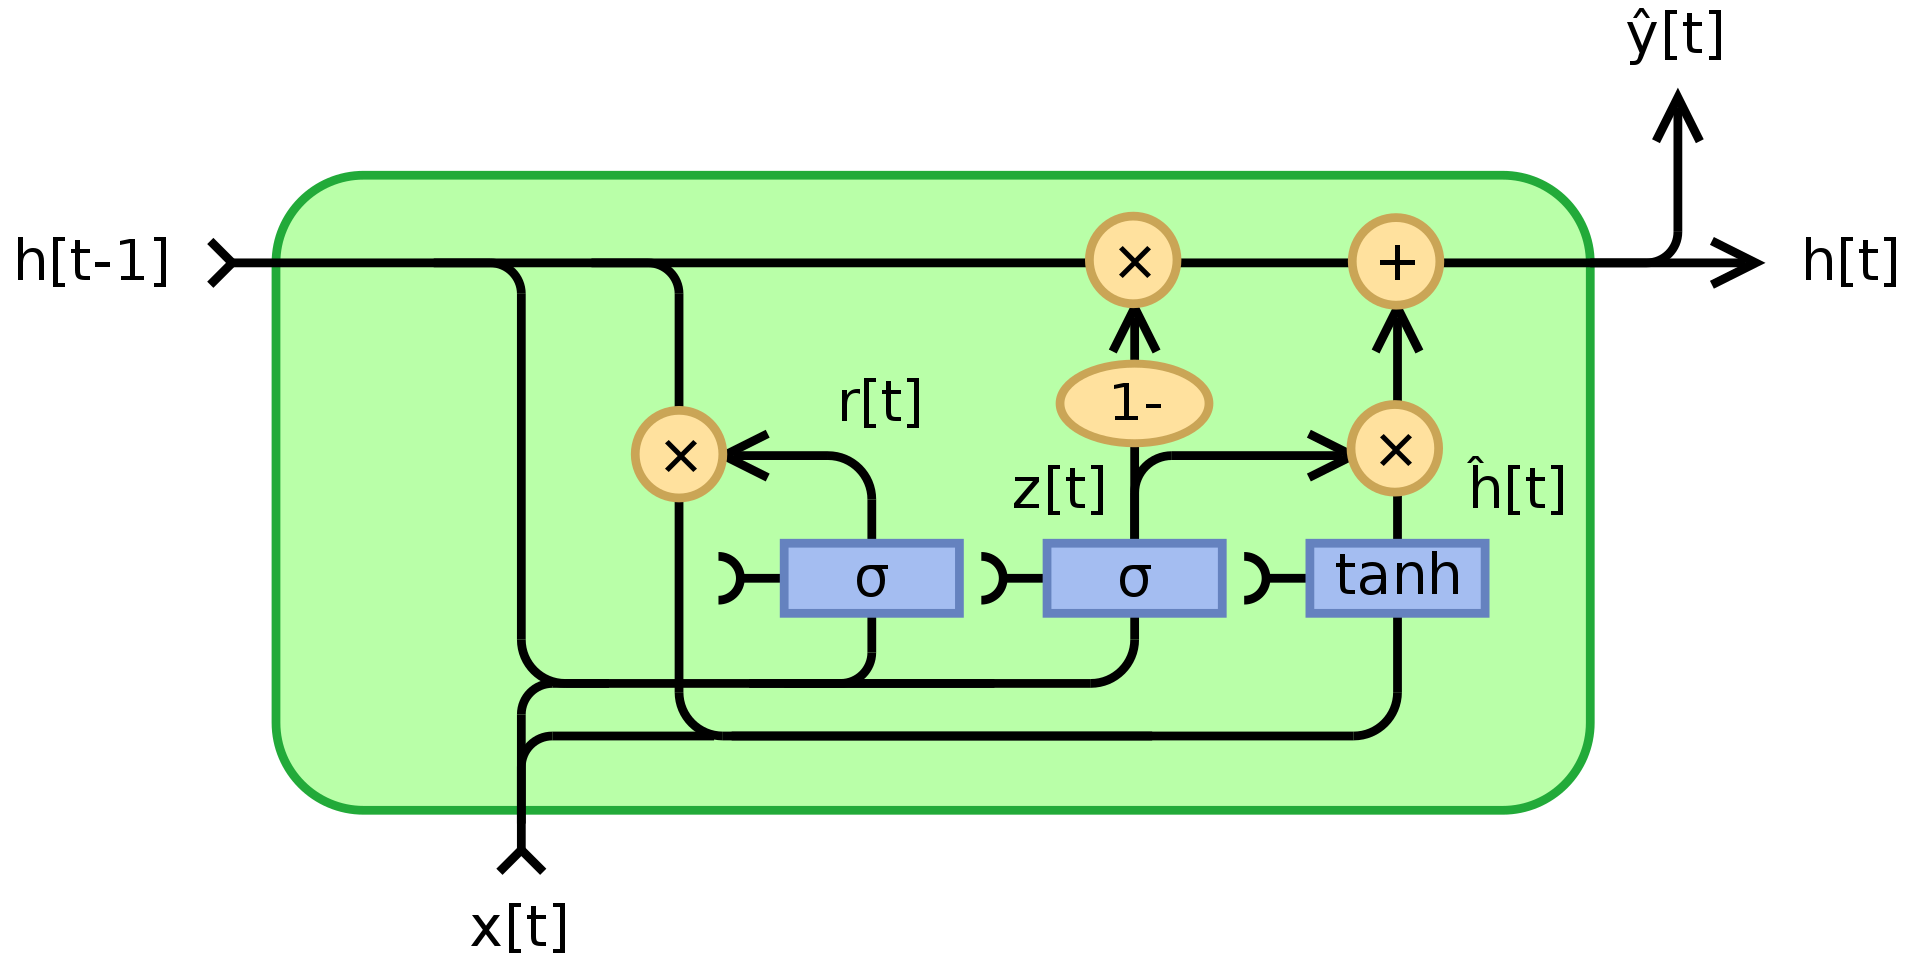
\includegraphics[width=\textwidth]{figs/GRU.png}\\
	        \scriptsize\href{https://en.wikipedia.org/wiki/Gated_recurrent_unit}{(Source)}
    \end{columns}
\end{frame}

\subsection{Advanced RNNs}
\begin{frame}{Recurrent networks}{Advanced architectures}
   \begin{columns}
 	   \column{.50\textwidth}
      		\begin{itemize}
	  	\item Attention networks
		\item Transformers (and visual transformers)
          	\item Encoder-decoder architectures
      	    \end{itemize}
 
 	   \column{.50\textwidth}
	    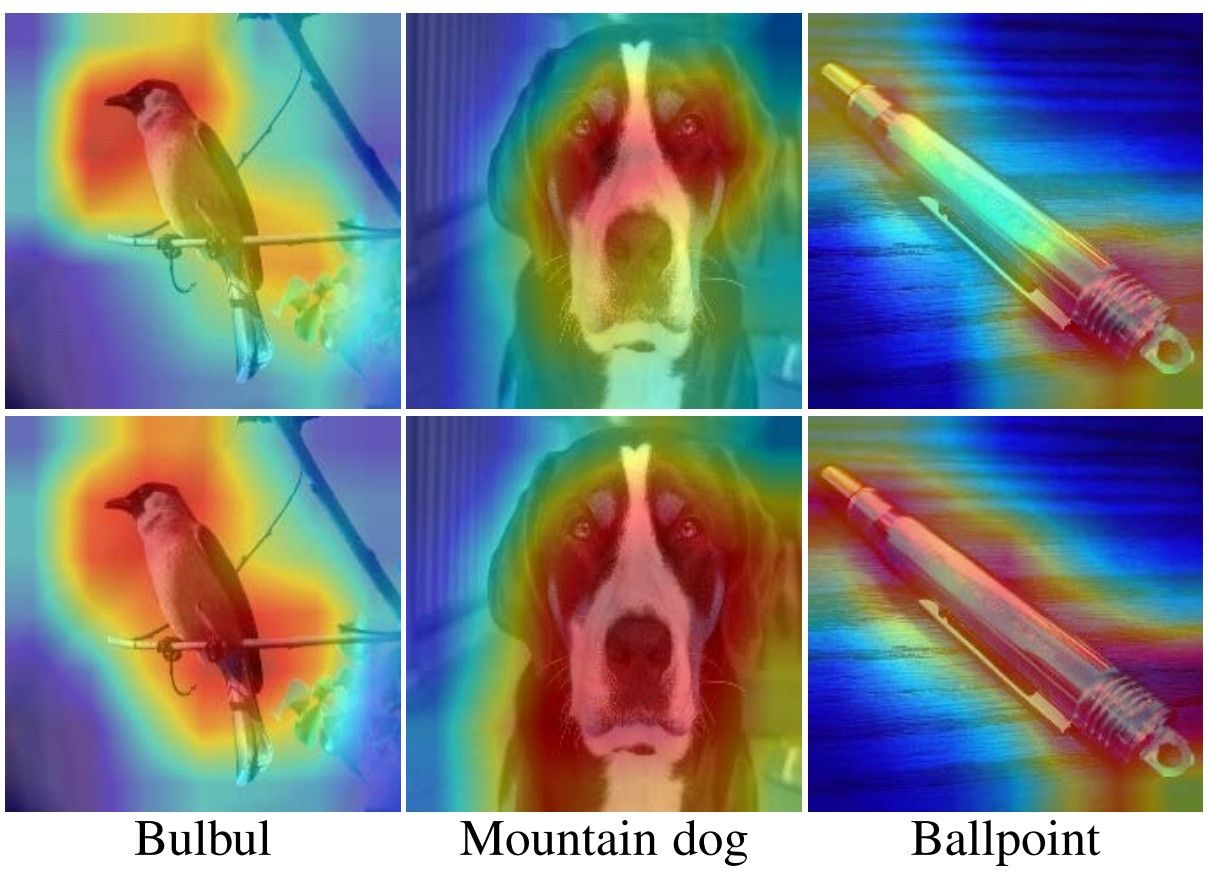
\includegraphics[width=\linewidth]{figs/attention.jpg}\\
	    \scriptsize\href{https://blog.paperspace.com/attention-mechanisms-in-computer-vision-cbam/}{(Source)}\\
    \end{columns}

\end{frame}

\subsection{RNNs cool applications}
\begin{frame}[plain,fragile]{Recurrent networks}{RNNs cool applications: language generation with a LSTM} 
    \small
    \begin{columns}
 	   \column{.50\textwidth}
       \begin{exampleblock}{Shakespeare}
\begin{verbatim}
PANDARUS:
Alas, I think he shall be come
approached and the day
When little srain would be
attain'd into being never fed,
And who is but a chain and
subjects of his death,
I should not sleep.
Second Senator:
They are away this miseries,
produced upon my soul,
Breaking and strongly should
be buried, when I perish
The earth and thoughts of
many states.
\end{verbatim}
       \end{exampleblock}

 	   \column{.50\textwidth}
       \begin{exampleblock}{Cervantes}
\begin{verbatim}
-pero me manda mal -respondió
el maererlino, que yo no será
mejor que se ha de ser de don
quijote, que no le
acompañasen, se vengaban de
haber tenido al cabo de los
cuales se venció de su escudero,
y el infierno que todos los
pasaron su hermosura, y a mí
me parece que se cuenta el
yelmo de la caballería, don
gregorio de la similacada al
caballo que de la mano, según la
señora dulcinea del toboso.
-no es bien -respondió sancho-,
\end{verbatim}
       \end{exampleblock}
    \end{columns}
\end{frame}


\begin{frame}{Recurrent networks}{RNNs cool applications: music synthesis} 
    \begin{columns}
 	   \column{.250\textwidth}
	DeepBach
    \begin{itemize}
        \item \href{https://www.youtube.com/watch?v=QiBM7-5hA6o}{(Video)}
        \item \href{http://proceedings.mlr.press/v70/hadjeres17a/hadjeres17a.pdf}{(Paper)}
        \item \href{https://github.com/Ghadjeres/DeepBach}{(Code)}
    \end{itemize}
 	   \column{.50\textwidth}
            \centering 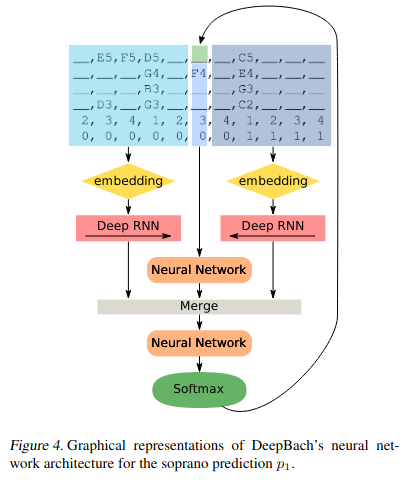
\includegraphics[width=\textwidth]{figs/bach.png}\\
	        \scriptsize\href{http://proceedings.mlr.press/v70/hadjeres17a/hadjeres17a.pdf}{(Source)}
    \end{columns}
\end{frame}


\section{Autoencoders}

\subsection{Autoencoders}

\begin{frame}{Autoencoders}{Autoencoders}
	\centering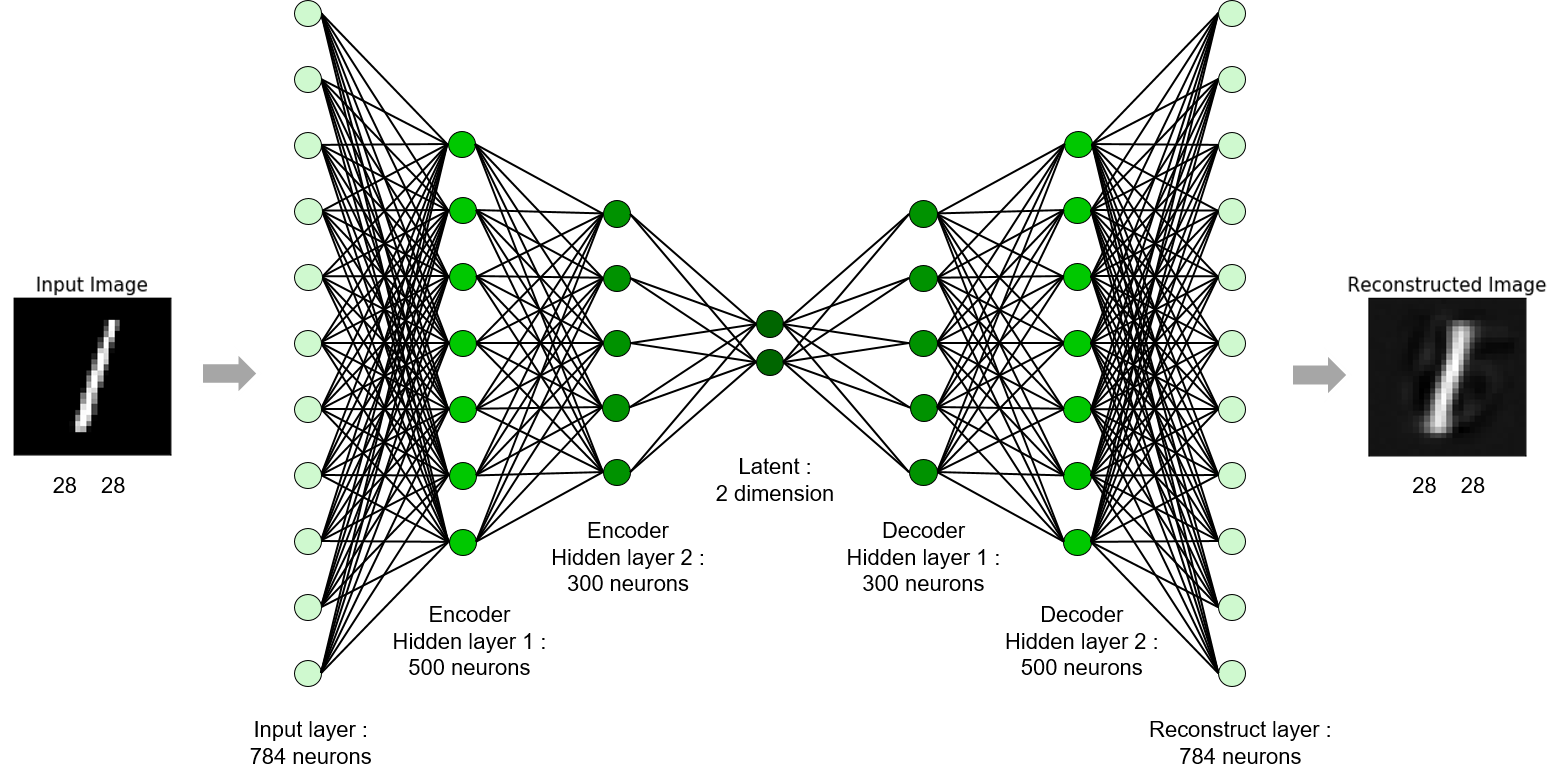
\includegraphics[width=0.75\linewidth]{figs/autoencoder.png}\\
	\centering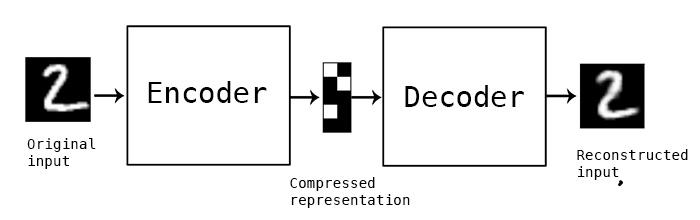
\includegraphics[width=0.3\linewidth]{figs/autoencoder2.png}\\
	\scriptsize\href{http://i-systems.github.io/HSE545/machine\%20learning\%20all/KIMM/06\_KIMM\_Autoencoder.html}{(Source)}
	\medskip

	\normalsize

	\begin{flushleft}
	Important concepts: \alert{latent space} and \alert{latent variables}
	\end{flushleft}
\end{frame}

\subsection{Autoencoders for anomaly detection}

\begin{frame}{Autoencoders}{Autoencoders for anomaly detection (I)}
	\documentclass[crop,tikz]{standalone}% 'crop' is the default for v1.0, before it was 'preview'

\usetikzlibrary{shapes,arrows}

\begin{document}


\tikzstyle{block} = [draw, rectangle, minimum height=3em, minimum width=6em]
\tikzstyle{sum} = [draw, circle, node distance=1cm]
\tikzstyle{input} = [coordinate]
\tikzstyle{output} = [coordinate]
\tikzstyle{pinstyle} = [pin edge={to-,thin,black}]

\begin{tikzpicture}[auto, node distance=2cm,>=latex']
 \node [input, name=input] {};
 \coordinate [right of=input, node distance=1.5cm] (sum){};
 %\node [sum, right of=input] (sum) {};
 \node [block, right of=sum] (autoencoder) {Autoencoder};
 \node [sum, right of=autoencoder, node distance=2.5cm] (resta) {$-$};
 \node [input, name=output, right of=resta, node distance = 2cm] {$-$};
 \coordinate [below of=autoencoder, node distance=1.5cm] (abajo){};
 %\node [block, right of=controller, node distance=3cm] (motor) {G$_{motor}$};
 %\node [block, right of=motor, pin={[pinstyle]above:Störningar},
 %       node distance=3cm] (system) {Dynamik$_{\varphi}$};

 %\draw [->] (controller) -- node[name=u] {$u$} (motor);
 %\node [output, right of=system] (output) {};
 %\node [block, below of=motor] (msystem) {Mätsystem};

	\draw [draw,->] (input) -- node {$\vec{x}$} (autoencoder);
 %\draw [->] (sum) -- node {$e$} (autoencoder);
	\draw [->] (autoencoder) -- node {$\vec{x}'$} (resta);
	\draw [->] (resta) -- node {$\epsilon$} (output);
	%\draw [->] (resta) -- node {$\epsilon=||\vec{x}'-\vec{x}'$||} (output);
	\draw [->] (sum) |- (abajo) -| (resta);
 %\draw [|-] (sum) -- node {} (abajo);
 %\draw [-|] (abajo) -- node {} (resta);

 %\draw [->] (system) -- node [name=y] {$\varphi$}(output);
 %\draw [->] (y) |- (msystem);
 %\draw [->] (msystem) -| node[pos=0.99] {$-$}  node [near end] {$\varphi_m$} (sum);
\end{tikzpicture}

\end{document} 

	\bigskip
	\alert{Reconstruction error} is an anomality measure
	\begin{itemize}
		\item A norm can be computed to provide a global measure (MAE/MSE), or ...
		\item ... keep reconstruction error as vector
	\end{itemize}
    PCA may be used, less powerfull than autoencoders
\end{frame}

\begin{frame}{Autoencoders}{Autoencoders for anomaly detection (II)}
	\centering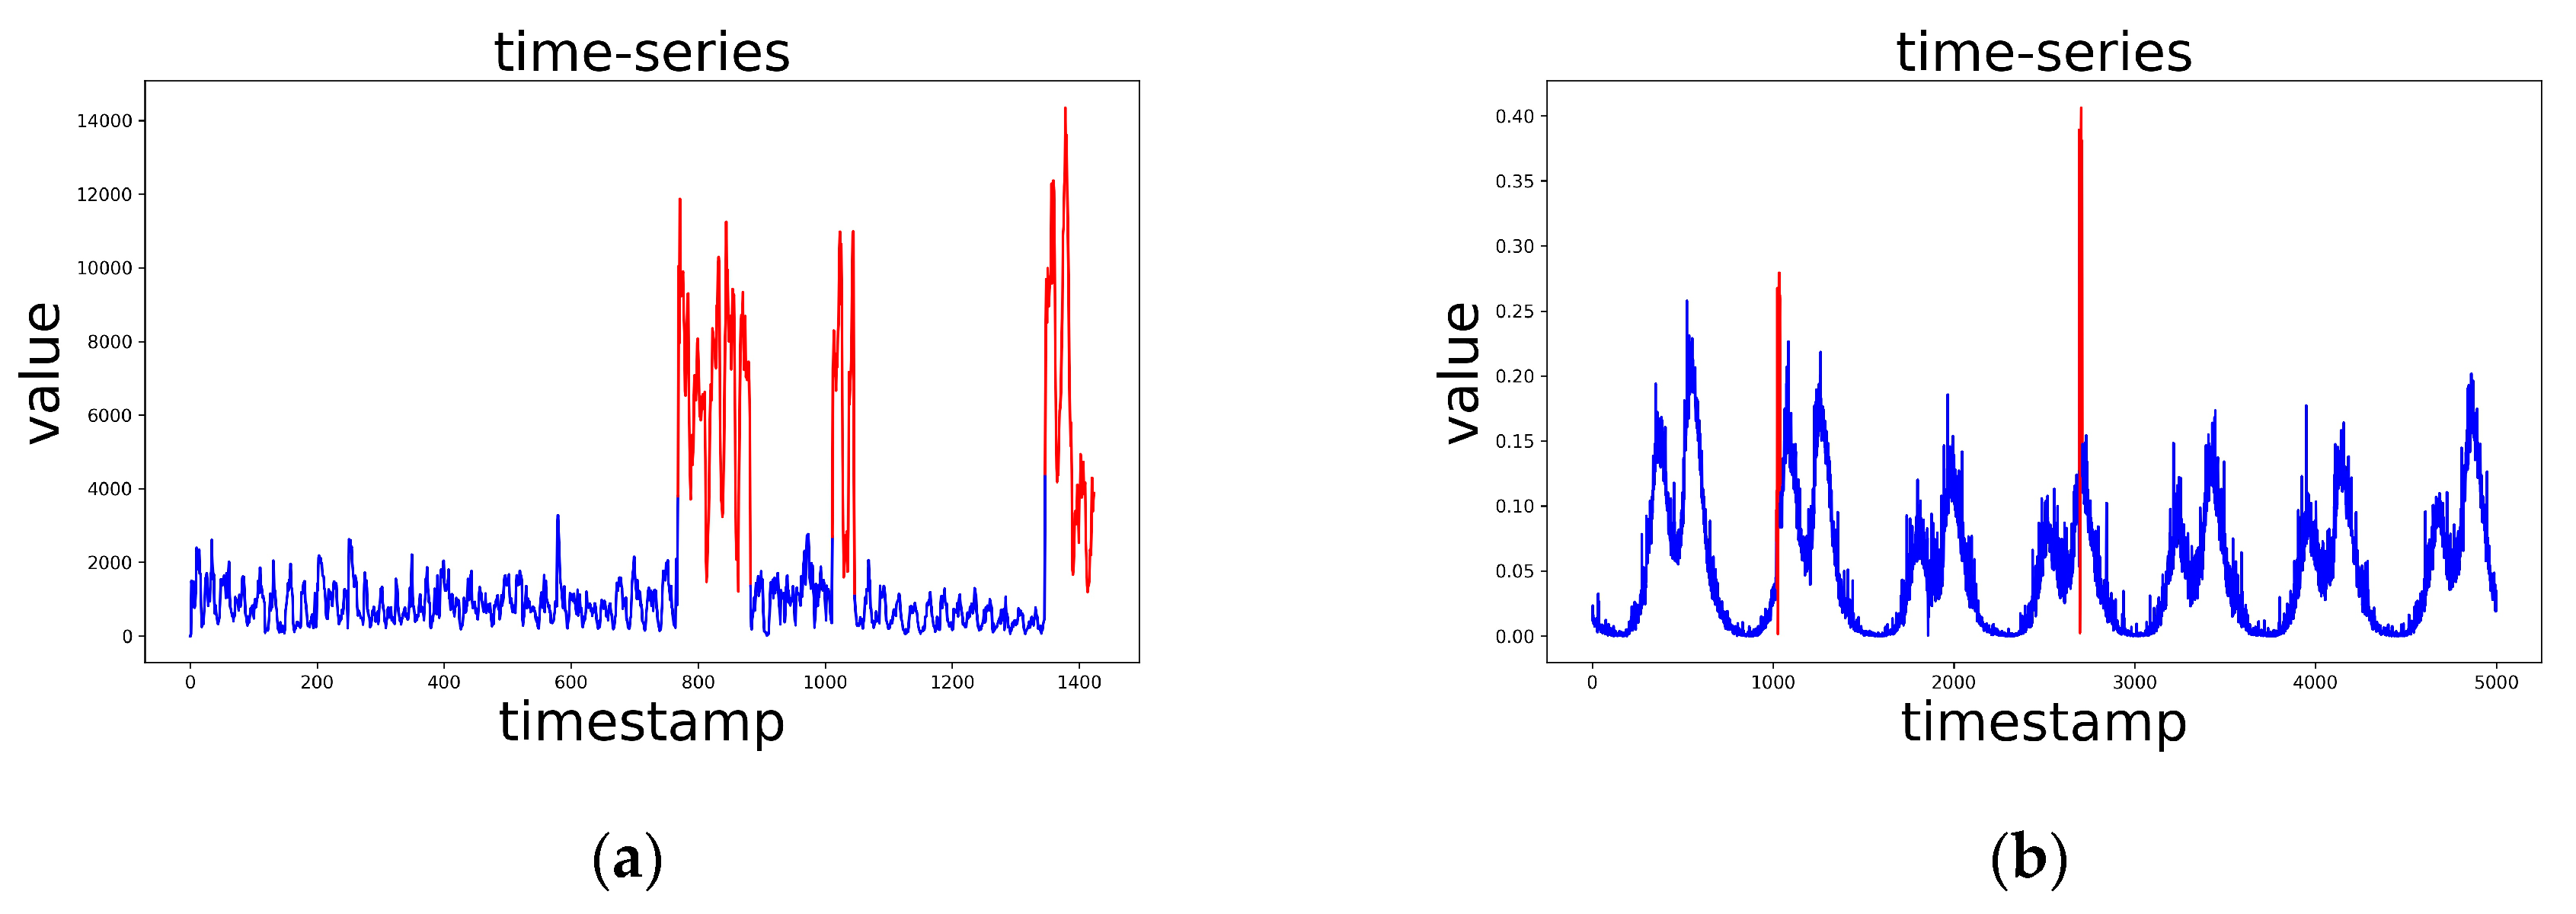
\includegraphics[width=0.75\linewidth]{figs/autoencoderts.png}\\
	\scriptsize\href{https://www.mdpi.com/1424-8220/20/13/3738}{(Source: Niu, Z.; Yu, K.; Wu, X. \textit{LSTM-Based VAE-GAN for Time-Series Anomaly Detection}. Sensors 2020, 20, 3738.)}

	\bigskip
	\begin{flushleft}
	\normalsize{
	Great flexibility to handle reconstruction error
	\begin{itemize}
		\item Trigger an alarm based on a threshold
		\item Analize the time-series
		\item Feed a classifier
	\end{itemize}
	}
	\end{flushleft}
\end{frame}

\subsection{Autoencoders as generative models}
\begin{frame}{Autoencoders}{Autoencoders as generative models (I)}
    \begin{columns}
 	   \column{.60\textwidth}
     Any autoencoder may be used as a generative model
	\begin{itemize}
		\item The decoder can reconstruct an instance from a latent space sample
	\end{itemize}

 	   \column{.40\textwidth}
	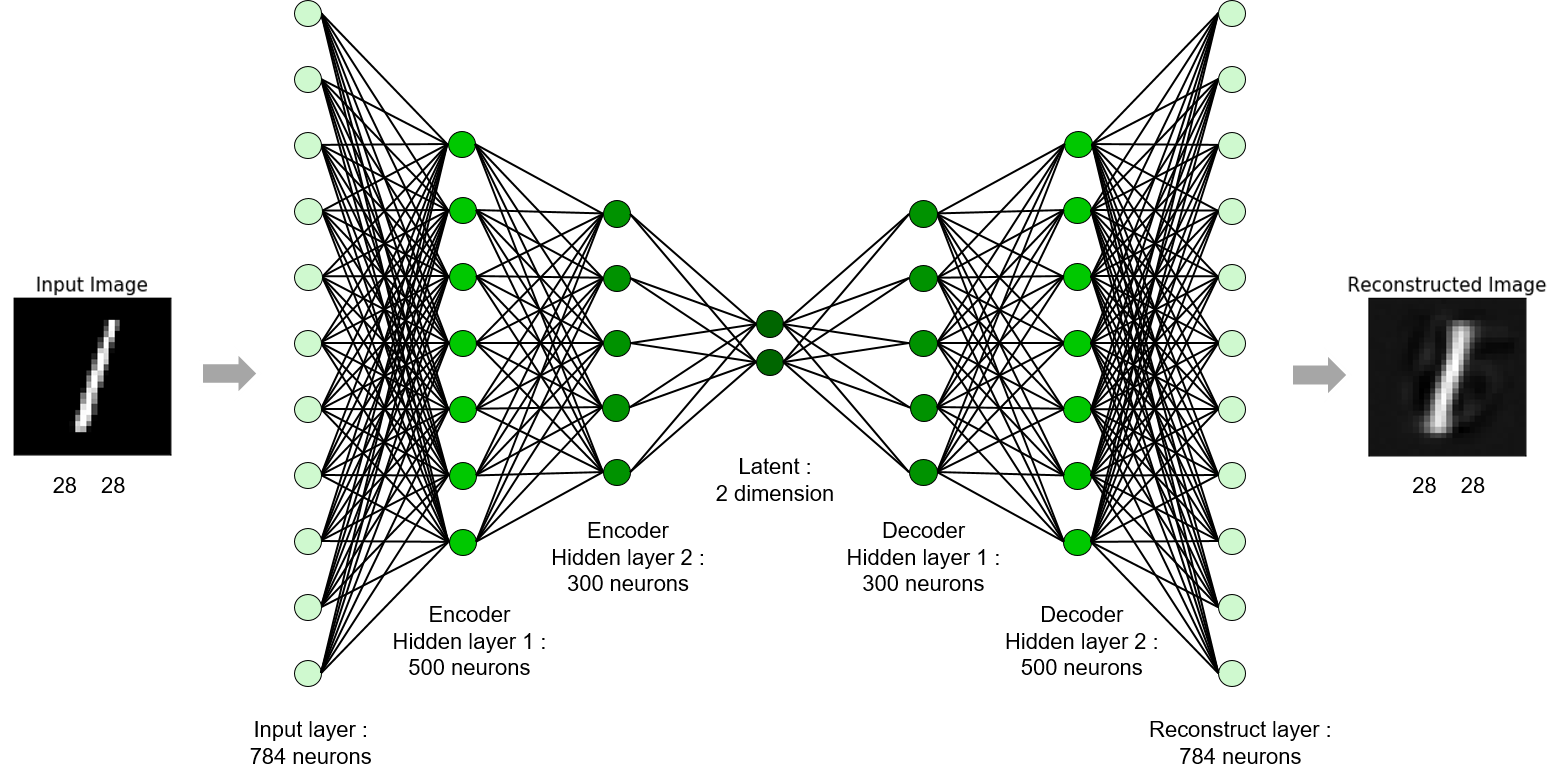
\includegraphics[width=\textwidth]{figs/autoencoder.png}\\
	\scriptsize\href{http://i-systems.github.io/HSE545/machine\%20learning\%20all/KIMM/06\_KIMM\_Autoencoder.html}{(Source)}
		
	\end{columns}

	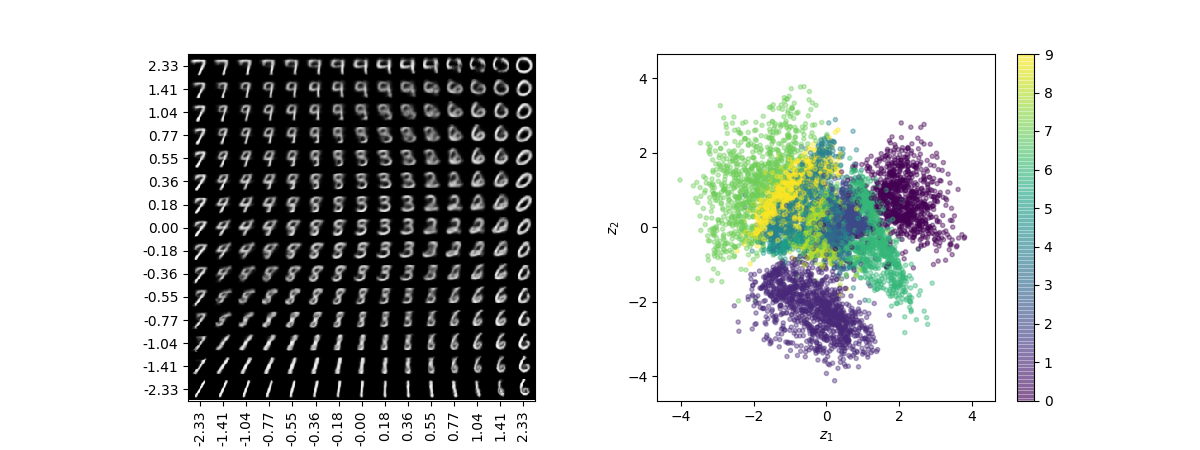
\includegraphics[width=\textwidth]{figs/latent2.png}\\
	\scriptsize\href{https://towardsdatascience.com/intuitively-understanding-variational-autoencoders-1bfe67eb5daf}{(Source)}
\end{frame}

\begin{frame}{Autoencoders}{Autoencoders as generative models (II)}
	Regular autoencoders are not a good choice for generative models

    \begin{columns}
 	   \column{.40\textwidth}
		\begin{figure}
	        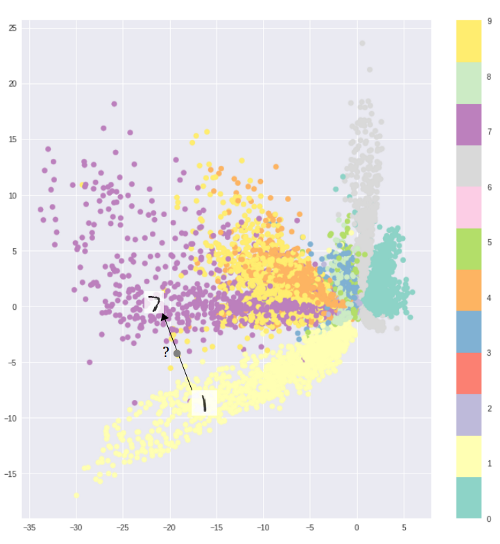
\includegraphics[width=\textwidth]{figs/latent.png}\\
		\scriptsize\href{https://towardsdatascience.com/intuitively-understanding-variational-autoencoders-1bfe67eb5daf}{(Source)}
		\end{figure}
    \end{columns}

\end{frame}

\section{Advanced topics}

\subsection{GAN}

\subsection{Advanced topics}
\begin{frame}{Advanced topics}{Generative networks: GAN (I)}
	\centering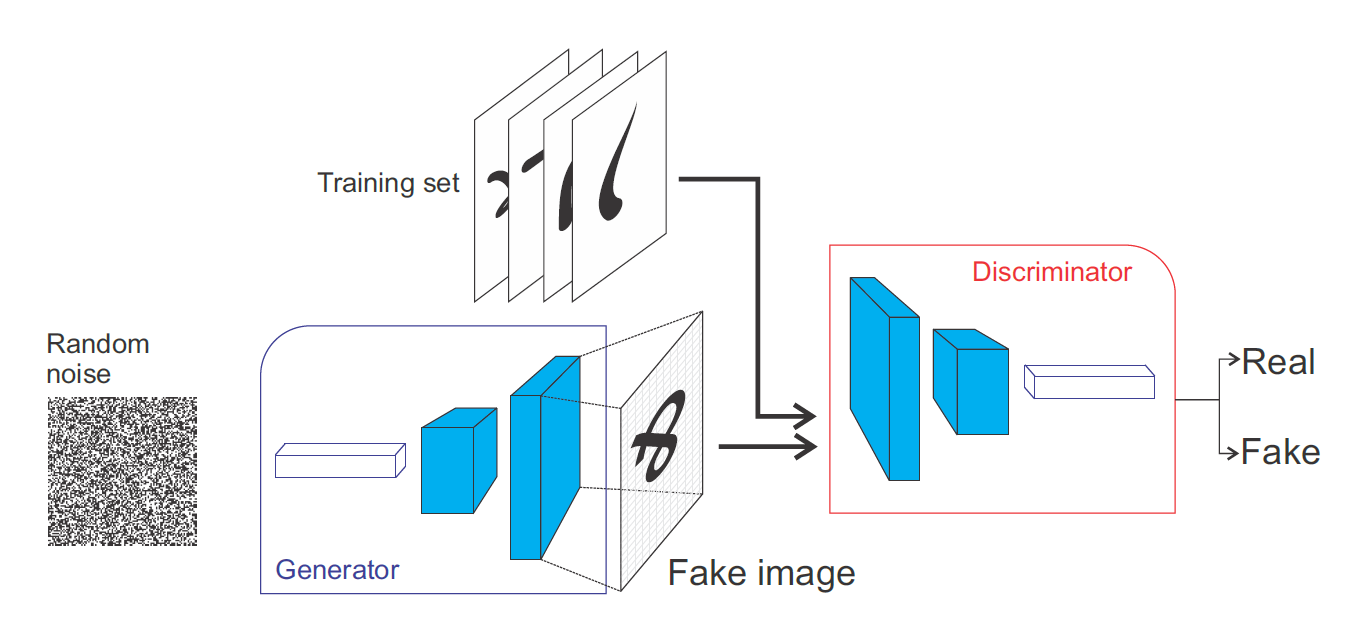
\includegraphics[width=0.7\linewidth]{figs/gan.png}\\
	\scriptsize\href{https://www.oreilly.com/library/view/java-deep-learning/9781788997454/60579068-af4b-4bbf-83f1-e988fbe3b226.xhtml}{(Source)}\\

    \normalsize
    \begin{flushleft}
   Examples:\\
    \begin{itemize}
        \item \href{https://thispersondoesnotexist.com/}{(Faces)}, \href{https://thisartworkdoesnotexist.com/}{(art)}, \href{http://www.thisworddoesnotexist.com/}{(Words)}, \href{https://thesecatsdonotexist.com/}{(cats)}
    \end{itemize}
    \end{flushleft}
\end{frame}

\begin{frame}{Advanced topics}{Generative networks: GAN (II)}
    \centering GauGAN \href{https://www.nvidia.com/en-us/studio/canvas/}{(Demo)}\\
	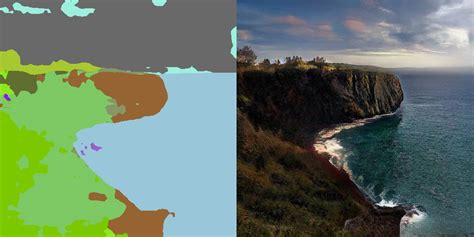
\includegraphics[width=0.9\linewidth]{figs/gaugan.jpeg}
\end{frame}

\subsection{VAE}
\begin{frame}{Advanced topics}{Variational Autoencoders (I)}
	\centering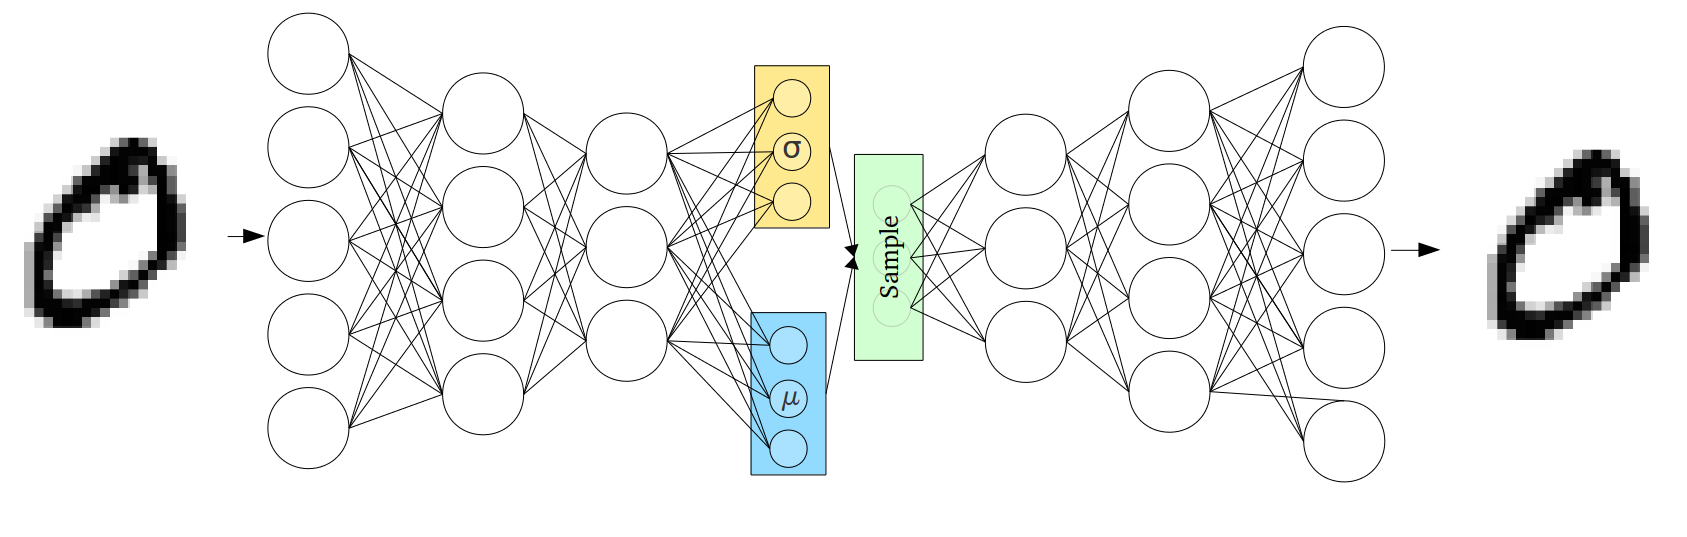
\includegraphics[width=0.85\linewidth]{figs/vae.png}\\
	\scriptsize\href{https://towardsdatascience.com/intuitively-understanding-variational-autoencoders-1bfe67eb5daf}{(Source)}

	\bigskip

	\flushleft
	\normalsize

	VAEs encodes latent variables as probability distributions
	\begin{itemize}
		\item Gaussian distributions with $\mu$ and $\sigma$
		\item Decoder sample the distributions
	\end{itemize}
\end{frame}

\begin{frame}{Advanced topics}{Variational Autoencoders (II)}
	\centering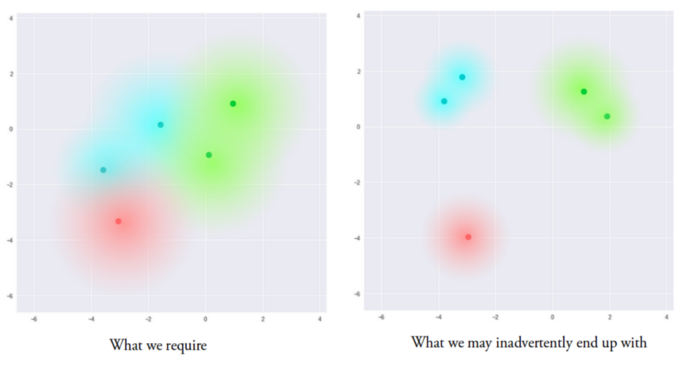
\includegraphics[width=0.6\linewidth]{figs/vae-kl.png}\\
	\scriptsize\href{https://towardsdatascience.com/intuitively-understanding-variational-autoencoders-1bfe67eb5daf}{(Source)}

	\smallskip

	\flushleft
	\normalsize

	We want a structured latent space
	\begin{itemize}
		\item Penalty based on \textit{Kullback-Leibler} (KL) divergence
			\begin{itemize}
				\item KL measures divergente between two probability distributions
			\end{itemize}
	\end{itemize}
\end{frame}

\begin{frame}{Advanced topics}{Variational Autoencoders: semantics (I)}
	Astonishing VAE feature: latent space has semantics!
	\centering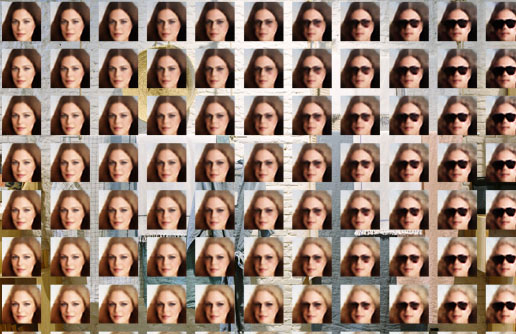
\includegraphics[width=0.7\linewidth]{figs/faces.jpg}\\
	\scriptsize\href{https://www.compthree.com/blog/autoencoder/}{(Source)}
\end{frame}

\begin{frame}{Advanced topics}{Variational Autoencoders: semantics (II)}
	Another incredible VAE property: 'semantic' arithmetic operations
	\centering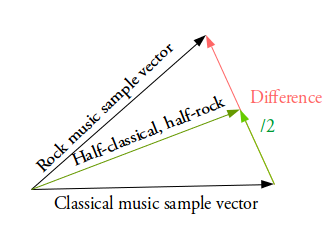
\includegraphics[width=0.3\linewidth]{figs/vector-vae1.png}\quad
	\centering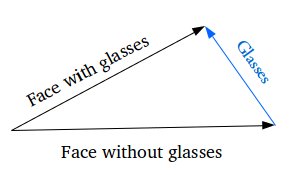
\includegraphics[width=0.3\linewidth]{figs/vector-vae2.png}\\
	\scriptsize\href{https://towardsdatascience.com/intuitively-understanding-variational-autoencoders-1bfe67eb5daf}{(Source)}

	\bigskip
	\normalsize
	\href{https://projector.tensorflow.org/}{(Embedding Projector)}
\end{frame}

\subsection{Generative models state-of-the-art}
\begin{frame}{Advanced topics}{Generative models state-of-the art}
	\centering Dall-E 2
    \bigskip
    \centering
    \begin{columns}
 	   \column{.50\textwidth}
	        A raccoon astronaut with the cosmos reflecting on the glass of his helmet dreaming of the stars\\\medskip
            
\includegraphics[width=0.8\linewidth]{figs/racoon.jpg}\\
	        \centering \scriptsize\href{https://bdtechtalks.com/2022/04/11/openai-dall-e-2/}{(Source)}

 	   \column{.50\textwidth}
	        Cosmic thoughts exploding\\\medskip
            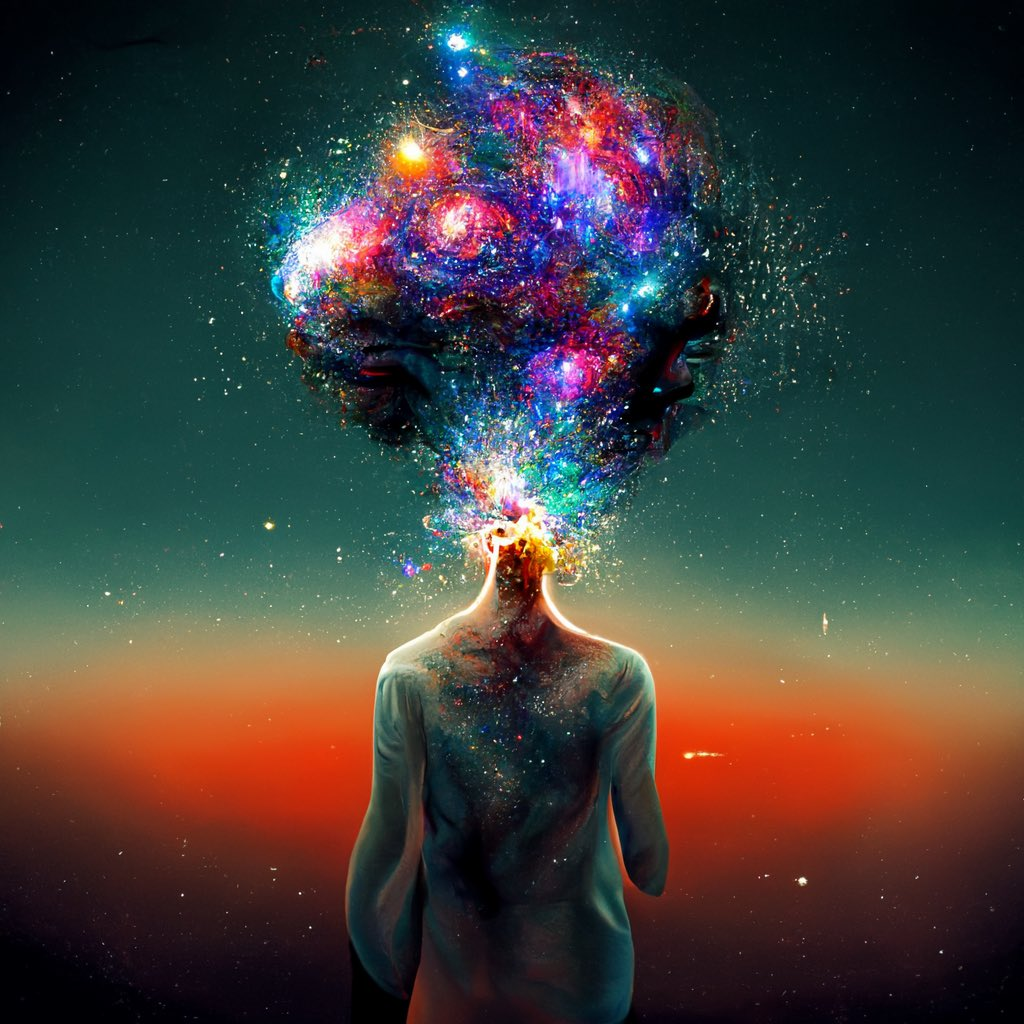
\includegraphics[width=0.8\linewidth]{figs/cosmic.jpg}\\
	        \centering \scriptsize\href{https://t.co/mfgrJkYiy9}{(Source)}
    \end{columns}
\end{frame}

\begin{frame}{Advanced topics}{Adversarial examples}
	\centering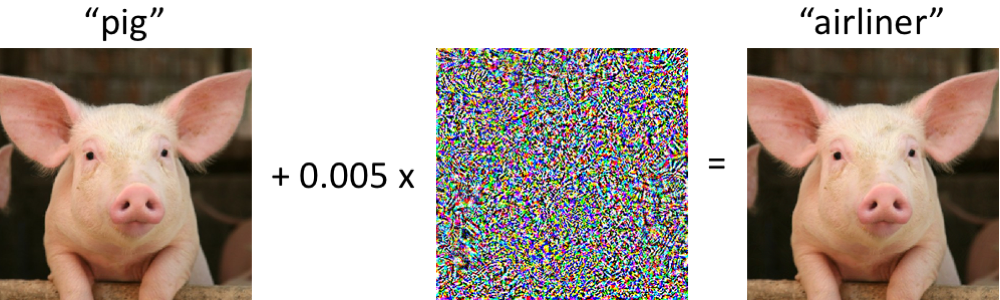
\includegraphics[width=0.7\linewidth]{figs/adversarial.png}\\
	\scriptsize\href{https://medium.com/attentive-ai/fooling-cnns-via-adversarial-examples-877a9e0ee84e}{(Source)}
\end{frame}


\end{document}
